% ==========================================================
% Relatório Final - Projeto Integrado em CD e IA (UEL)
% Projeto: Redes Neurais Convolucionais Explicáveis na
%          Classificação de Imagens de Resíduos
% Compile com: pdflatex (ou latexmk -pdf)
% ==========================================================
\documentclass[11pt,a4paper]{article}

% ---------- Pacotes ----------
\usepackage[utf8]{inputenc}
\usepackage[T1]{fontenc}
\usepackage[brazil]{babel}
\usepackage{amsmath,amssymb}
\usepackage{graphicx}
\usepackage{booktabs}
\usepackage{multirow}
\usepackage{enumitem}
\usepackage{xcolor}
\usepackage{caption}
\usepackage{tikz}
\usetikzlibrary{arrows.meta,positioning}
\usepackage[top=3.5cm,bottom=3cm,left=3cm,right=3cm,headheight=2cm]{geometry}
\usepackage{fancyhdr}
\usepackage{microtype}
\usepackage[hidelinks]{hyperref}

% ----------- Cabeçalho -----------
\pagestyle{fancy}
\fancyhf{}
\renewcommand{\headrulewidth}{0pt}

% Expande o cabeçalho 1.2cm para a esquerda e 1.2cm para a direita além da largura do texto
\fancyheadoffset[L,R]{1.2cm}

\fancyhead[L]{%
	\begin{minipage}[b]{0.68\headwidth}
		\raggedright
		{\large\bfseries Ciência de Dados e Inteligência Artificial}\\
		{\small\textbf{Disciplina:} Projeto Integrado em Ciência de Dados e Inteligência Artificial}\\
		{\small\textbf{Professor:} Felipe Kenji Nakano}
	\end{minipage}%
}
\fancyhead[R]{%
	\IfFileExists{logo_uel.png}{
\includegraphics[height=1.3cm]{logo_uel.png}}{}%
}
\fancyfoot[C]{\thepage}

% ---------- Ajustes e macros ----------
\setlist[itemize]{leftmargin=1.5cm}
\setlist[enumerate]{leftmargin=1.5cm}
\renewcommand{\refname}{Referências}
\captionsetup{font=small,labelfont=bf,labelsep=period}
\graphicspath{{fig/}}
\setlength{\emergencystretch}{2em}
\renewcommand{\topfraction}{0.9}
\renewcommand{\bottomfraction}{0.7}
\renewcommand{\textfraction}{0.07}
\renewcommand{\floatpagefraction}{0.95}

\begin{document}
	
	\begin{center}
		{\Large\bfseries Relatório final}
	\end{center}
	\vspace{1em}
	
	% ---------- Grupo ----------
	\section*{Grupo}
	\begin{itemize}
		\item \textbf{Integrantes:} Guilherme Nascimento Braga, Keila Kaori Horiye, Luanna Garla
		\item \textbf{Título do projeto:} Redes Neurais Convolucionais Explicáveis na Classificação de Imagens de Resíduos
	\end{itemize}
	
	% ---------- Resumo ----------
	\begin{quote}
		\small
		\textbf{Resumo.} A classificação automática de resíduos por visão computacional é limitada por dois problemas que se reforçam mutuamente: os conjuntos de dados públicos são fragmentados, com rótulos, resoluções e vocabulários incompatíveis, e os modelos resultantes são opacos, o que impede saber se a decisão se apoia no resíduo ou em artefatos do cenário. Este trabalho construiu um \textit{benchmark} integrado e auditável a partir de quatro bases públicas, com harmonização semântica assistida por CLIP e deduplicação por \textit{hash} exato e perceptual, e avaliou a generalização de redes convolucionais em um protocolo de avaliação cruzada entre domínios. O modelo treinado no conjunto combinado (EfficientNet-B0, oito classes) obteve a melhor média nos dois conjuntos externos que não participaram de nenhum treinamento (0,769 de acurácia balanceada restrita), contra 0,732 de MobileNetV2 e 0,732 de ResNet18. O Grad-CAM foi usado como instrumento de auditoria: antes da curadoria, o modelo classificava uma luva olhando para o fundo da imagem; depois dela, os mapas passaram a destacar o objeto, ainda que falhas residuais permaneçam. O modelo foi exportado para ONNX, verificado contra o \textit{checkpoint} em 4.212 imagens e implantado em um aplicativo Android que calcula o Grad-CAM no próprio aparelho.
		
		\smallskip
		\noindent\textbf{Palavras-chave:} classificação de resíduos; redes neurais convolucionais; Grad-CAM; generalização entre domínios; integração de conjuntos de dados.
	\end{quote}
	
	% ==========================================================
	\section{Introdução}
	
	\textbf{Contexto e problema.} A geração global de resíduos sólidos continua crescendo: a projeção do Banco Mundial indica um aumento de 2,1 bilhões para 3,4 bilhões de toneladas por ano até 2050 \cite{kaza2018}. A triagem desses materiais é uma etapa crítica do manejo: consome tempo e expõe os trabalhadores a riscos de insalubridade, além de ser suscetível a erro humano. A automação por visão computacional é uma alternativa natural, e a literatura recente acumulou um grande número de trabalhos que aplicam aprendizado profundo à classificação e à detecção de resíduos \cite{fotovvatikhah2025,bawankule2023,shourie2024}.
	
	\textbf{Lacuna na literatura.} Apesar do volume de publicações, a revisão sistemática de Fotovvatikhah et al. \cite{fotovvatikhah2025} mostra que a maioria dos estudos avalia o modelo em um único conjunto de dados, com uma única distribuição de captura, e reporta apenas métricas no domínio de treino. Bawankule et al. \cite{bawankule2023}, cuja base de 12 classes foi o ponto de partida deste trabalho, e Shourie et al. \cite{shourie2024} seguem o mesmo padrão. Dessa revisão emergem dois problemas que este trabalho se propôs a enfrentar.
	
	O primeiro é a \emph{falta de integração entre conjuntos de dados}. As bases públicas diferem no vocabulário de rótulos (a mesma embalagem longa vida é \texttt{tetra\_pack} em uma base e \texttt{paper} ou \texttt{cardboard} em outra), no tamanho e na resolução das imagens, no número de classes e no protocolo de captura. Sem harmonização, um modelo treinado em uma base aprende atalhos específicos daquela fonte --- fundo, iluminação, enquadramento --- e falha quando o domínio muda \cite{geirhos2020,babe2025}. Pior: a mesma imagem pode aparecer em bases diferentes, com nome de arquivo distinto, e contaminar a divisão treino/teste, inflando artificialmente qualquer comparação.
	
	O segundo é a \emph{baixa confiança no uso desses modelos}, consequência de sua natureza de caixa-preta. Uma acurácia alta não diz \emph{por que} o modelo acertou nem permite inspecionar \emph{quando} ele falha. Em um domínio em que o descarte incorreto tem consequência ambiental e econômica, essa opacidade é um obstáculo prático à adoção.
	
	\textbf{Objetivos.} O objetivo geral foi desenvolver e avaliar um classificador de resíduos baseado em redes neurais convolucionais que fosse, ao mesmo tempo, generalizável entre fontes de imagens e interpretável. Os objetivos específicos foram: (i) construir um conjunto de dados integrado, com rótulos harmonizados e sem vazamento entre treino, validação e teste; (ii) definir um protocolo de avaliação cruzada que medisse a transferência entre domínios de forma justa; (iii) comparar arquiteturas convolucionais sob o mesmo protocolo; e (iv) auditar as predições com Grad-CAM e levar o modelo para um aplicativo móvel.
	
	\textbf{Contribuições.} As contribuições do trabalho são:
	\begin{itemize}
		\item um \textit{pipeline} reprodutível de curadoria que indexa 35.603 imagens, agrupa-as em 32.482 clusters de conteúdo por MD5, dHash e pHash, exclui 31 clusters ambíguos (83 imagens) --- resultando em 32.451 clusters --- e produz quatro projeções por fonte e um conjunto combinado de 15.707 imagens em oito classes;
		\item um protocolo de avaliação cruzada com 24 pares modelo $\times$ alvo, incluindo dois conjuntos externos que não participaram de nenhum treinamento (Garbage12, com 12.450 imagens, e RealWaste, com 4.752), com métricas que separam acurácia, cobertura e capacidade de nomear classes ausentes;
		\item uma comparação controlada de EfficientNet-B0, MobileNetV2 e ResNet18, rastreada em MLflow, que mostra a vantagem média da primeira e o custo-benefício da segunda;
		\item uma auditoria de explicabilidade com Grad-CAM que documenta o viés de fundo antes da curadoria e a melhora depois dela, além de um aplicativo Android que executa a classificação e o Grad-CAM localmente, sem rede.
	\end{itemize}
	
	\textbf{Organização.} A Seção~\ref{sec:background} apresenta a fundamentação teórica e os trabalhos relacionados. A Seção~\ref{sec:pipeline} descreve o \textit{pipeline} de curadoria, treinamento, otimização e explicabilidade. A Seção~\ref{sec:metodologia} detalha os conjuntos de dados, os modelos, as métricas e o protocolo experimental. A Seção~\ref{sec:resultados} discute os resultados, e a Seção~\ref{sec:conclusao} conclui o trabalho.
	
	% ==========================================================
	\section{Fundamentação Teórica e Trabalhos Relacionados}
	\label{sec:background}
	
	Nesta seção, formalizamos a tarefa de classificação de imagens, o método Grad-CAM e o aprendizado por transferência, e situamos o trabalho diante da literatura.
	
	\subsection{Formalização do problema}
	
	Seja $\mathcal{X} \subset \mathbb{R}^{H \times W \times 3}$ o espaço de imagens e $\mathcal{Y} = \{1, \dots, 8\}$ o conjunto de oito classes de resíduos adotado neste trabalho. Dado um conjunto rotulado $L = \{(\mathbf{x}_q, y_q)\}_{q=1}^{n}$, com $\mathbf{x}_q \in \mathcal{X}$ e $y_q \in \mathcal{Y}$, busca-se uma função $f : \mathcal{X} \rightarrow \mathcal{Y}$, parametrizada por uma CNN, que minimize o risco empírico
	\begin{equation}
		\hat{R}(f) = \frac{1}{n} \sum_{q=1}^{n} \ell\big(f(\mathbf{x}_q), y_q\big),
		\label{eq:risco}
	\end{equation}
	em que $\ell$ é a entropia cruzada. Como as classes são desbalanceadas, o critério de seleção de modelo não é a acurácia, mas o Macro-F1, definido na Seção~\ref{sec:metricas}.
	
	O ponto central deste trabalho não é a minimização de~\eqref{eq:risco} em uma única distribuição, mas o comportamento sob \emph{mudança de domínio}. Seja $P_S(\mathbf{x}, y)$ a distribuição de treino e $P_T(\mathbf{x}, y)$ a de um conjunto alvo. Em geral $P_S \neq P_T$, porque as fontes diferem em cenário, iluminação, resolução e até no vocabulário de rótulos. A avaliação cruzada mede o desempenho de $f$ treinada em $P_S$ e aplicada a $P_T$, e é por isso que a integridade da divisão entre fontes é parte do método, e não uma etapa de pré-processamento acessória.
	
	Como os vocabulários dos modelos e dos alvos não coincidem, seja $\mathcal{C}_m$ o conjunto de classes de um modelo e $\mathcal{C}_t$ o de um alvo. A avaliação restrita usa a interseção $\mathcal{S} = \mathcal{C}_m \cap \mathcal{C}_t$ e o conjunto de imagens cuja classe verdadeira pertence a $\mathcal{C}_m$, denotado por \emph{elegível}. A cobertura é a fração elegível do alvo, e a acurácia de implantação penaliza como erro toda imagem cuja classe o modelo não sabe nomear.
	
	\subsection{Aprendizado por transferência}
	
	Todas as redes foram inicializadas com pesos pré-treinados na ImageNet-1k e ajustadas em duas etapas. Na primeira, o \textit{backbone} permanece congelado e apenas a cabeça de classificação é treinada por três épocas (\emph{warmup}); na segunda, todos os parâmetros são liberados e ajustados com \emph{fine-tuning}. O descongelamento gradual é uma receita consolidada na literatura de transferência de aprendizado \cite{howardruder2018}: ele evita que gradientes grandes destruam as representações pré-treinadas nas primeiras atualizações e estabiliza a cabeça recém-inicializada antes de o \textit{backbone} começar a se mover. A mesma receita foi aplicada às três arquiteturas, de modo que a comparação não mistura diferenças de cronograma de treinamento.
	
	\subsection{Grad-CAM}
	
	O Grad-CAM \cite{selvaraju2017} produz um mapa de calor que indica as regiões da imagem mais relevantes para a classe $c$. Seja $y^c$ o escore da classe $c$ antes do \textit{softmax} e $A^k$ o $k$-ésimo mapa de ativação da última camada convolucional, com $Z$ posições espaciais. Os pesos de importância de cada mapa são
	\begin{equation}
		\alpha_k^c = \frac{1}{Z} \sum_{i} \sum_{j} \frac{\partial y^c}{\partial A^k_{ij}},
		\label{eq:gradcam-alpha}
	\end{equation}
	e o mapa de calor resultante é
	\begin{equation}
		L^c_{\text{Grad-CAM}} = \operatorname{ReLU}\!\left( \sum_{k} \alpha_k^c A^k \right).
		\label{eq:gradcam}
	\end{equation}
	
	Para as três arquiteturas usadas aqui, a cabeça é uma única camada linear após o \emph{pooling} global. Nesse caso, o gradiente do escore em relação ao vetor \emph{pooled} é exatamente a linha $c$ da matriz de pesos da cabeça, e o mapa pode ser calculado no dispositivo sem motor de gradientes, como
	\begin{equation}
		L^c = \operatorname{ReLU}\!\left( \sum_{k} W_{c,k}\, F_k \right),
		\label{eq:gradcam-linear}
	\end{equation}
	em que $F_k$ é o mapa de ativação e $W_{c,k}$ o peso correspondente. Essa identidade foi verificada numericamente contra o autograd e é o que viabiliza o Grad-CAM dentro do aplicativo Android. Ela não vale para arquiteturas cuja cabeça tenha mais de uma camada com ativação no meio --- o caso do MobileNetV3, descartado por esse motivo (Seção~\ref{sec:modelos}).
	
	\subsection{Trabalhos relacionados}
	
	\textbf{Classificação de resíduos e revisões sistemáticas.} A revisão de Fotovvatikhah et al. \cite{fotovvatikhah2025} organiza a área em classificação, detecção e segmentação, e observa que a comparabilidade entre estudos é baixa: cada trabalho usa uma base própria, um recorte de classes próprio e, muitas vezes, um protocolo de divisão próprio. Bawankule et al. \cite{bawankule2023} disponibilizaram uma base de 15.617 imagens em 12 classes, originalmente anotada no formato YOLO, que se tornou a base inicial deste projeto. Shourie et al. \cite{shourie2024} usam VGG16 para separar material orgânico de reciclável. Em comum, esses trabalhos reportam acurácia alta no domínio de treino e não avaliam a transferência para outras fontes.
	
	\textbf{Mudança de domínio em resíduos.} O trabalho de Babé et al. \cite{babe2025} é o mais próximo do nosso em espírito: cinco bases de resíduos, treino em uma e teste nas demais, com modelos de fundação e ajuste eficiente. Os autores relatam que aumentos de dados simples não melhoraram a generalização entre bases. Single et al. \cite{single2023}, ao introduzirem o RealWaste, medem o custo da mudança de cenário: modelos treinados em imagens de estúdio chegam a aproximadamente 50\% em ambiente real, enquanto o treino com imagens reais eleva o desempenho a 89,19\%. TrashBox \cite{kumsetty2022} explora justamente o cenário com objetos em \textit{clutter}. Esses resultados motivam um protocolo em que o teste externo é obrigatório e separado do ajuste de hiperparâmetros.
	
	\textbf{Atalhos aprendidos e o papel do fundo.} Geirhos et al. \cite{geirhos2020} descrevem o aprendizado de atalhos: a rede pode usar regularidades espúrias do conjunto --- textura do fundo, marca d'água, enquadramento --- que funcionam no domínio de treino e falham fora dele. No domínio de resíduos, Azzahra et al. \cite{azzahra2026} mostram que remover o fundo \emph{reduziu} a acurácia de um classificador de seis classes, o que indica que o fundo carrega contexto útil e que a solução não é simplesmente apagá-lo, mas garantir que o modelo não dependa dele. O Grad-CAM é usado neste trabalho precisamente para verificar de onde vem a decisão.
	
	\textbf{Integração de bases.} O GlobalWasteData \cite{ijaz2026} reúne cerca de vinte bases públicas em 89.807 imagens, 14 categorias e 68 subclasses, com filtragem de qualidade e remoção de duplicatas. Ele mostra que a integração de bases já é uma frente ativa; a diferença do nosso trabalho está no protocolo: a integração é acompanhada de uma garantia de isolamento entre clusters de conteúdo e de uma avaliação em que o teste de uma fonte nunca aparece no treino de outra.
	
	\textbf{Explicabilidade.} O Grad-CAM é usado na literatura de resíduos sobretudo como ilustração qualitativa de acertos. Aqui ele tem papel de auditoria: é a ferramenta que revelou o viés de fundo do primeiro modelo e que orientou a reconstrução do conjunto de dados. Essa diferença de uso --- explicação como diagnóstico, não como figura --- é uma das contribuições metodológicas do trabalho.
	
	% ==========================================================
	\section{Pipeline e Métodos Propostos}
	\label{sec:pipeline}
	
	\subsection{Visão geral}
	
	Não propomos uma nova arquitetura de rede. A contribuição é um \textit{pipeline} composto por três etapas: curadoria anti-vazamento dos dados, treinamento controlado com avaliação cruzada e explicabilidade com implantação móvel. A Figura~\ref{fig:pipeline} resume o fluxo, que é implementado como um grafo DVC de cinco estágios e reprodutível a partir das fontes brutas.
	
	\begin{figure}[htbp]
		\centering
		\begin{tikzpicture}[
			box/.style={draw, rounded corners=2pt, align=center, font=\footnotesize,
				minimum height=1.15cm, text width=3.25cm, fill=blue!4, draw=black!55},
			arr/.style={-{Latex[length=2mm]}, thick, draw=black!60}
			]
			\node[box] (a) at (0,0) {Quatro bases públicas\\35.603 imagens\\indexadas};
			\node[box] (b) at (4.4,0) {Harmonização de rótulos\\e curadoria com CLIP};
			\node[box] (c) at (8.8,0) {Deduplicação\\MD5, dHash e pHash};
			\node[box] (d) at (8.8,-2.2) {Registro \mbox{global} de \textit{splits}\\32.451 clusters};
			\node[box] (e) at (4.4,-2.2) {Quatro projeções\\por fonte (35.520)};
			\node[box] (f) at (0,-2.2) {Dataset combinado\\15.707 imagens\\8 classes};
			\node[box] (g) at (0,-4.4) {Treino controlado\\B0, MobileNetV2\\e ResNet18};
			\node[box] (h) at (4.4,-4.4) {Avaliação cruzada\\4 modelos $\times$ 6 alvos};
			\node[box] (i) at (8.8,-4.4) {Grad-CAM e\\aplicativo Android};
			\draw[arr] (a) -- (b);
			\draw[arr] (b) -- (c);
			\draw[arr] (c) -- (d);
			\draw[arr] (d) -- (e);
			\draw[arr] (e) -- (f);
			\draw[arr] (f) -- (g);
			\draw[arr] (g) -- (h);
			\draw[arr] (h) -- (i);
		\end{tikzpicture}
		\caption{Pipeline do projeto. O registro global de \textit{splits} é a autoridade única sobre a que divisão cada cluster de conteúdo pertence; as projeções por fonte e o conjunto combinado são derivados dele.}
		\label{fig:pipeline}
	\end{figure}
	
	\subsection{Harmonização de rótulos}
	
	O primeiro obstáculo foi o vocabulário. As quatro bases usam nomes diferentes para o mesmo material e o mesmo nome para materiais diferentes. A Tabela~\ref{tab:rotulos} resume as decisões. Nomes sinônimos foram unificados preservando o sentido da classe (por exemplo, \texttt{tin\_can} passou a \texttt{metal}, que é o nome usado pela maioria das bases); classes heterogêneas ou sem padrão foram excluídas; e materiais que apareciam diluídos em outras classes foram isolados.
	
	\begin{table}[htbp]
		\centering
		\small
		\caption{Harmonização dos rótulos entre as quatro fontes. Os rótulos marcados como excluídos não entram no conjunto combinado de oito classes.}
		\label{tab:rotulos}
		\setlength{\tabcolsep}{4pt}
		\begin{tabular}{p{3.8cm}p{3.0cm}p{2.8cm}p{4.2cm}}
			\toprule
			\textbf{Rótulo de origem} & \textbf{Fonte} & \textbf{Rótulo canônico} & \textbf{Tratamento} \\
			\midrule
			\texttt{bottle}, \texttt{soft\_plastic} & Roboflow & \texttt{plastic} & renomeado \\
			\texttt{tin\_can} & Roboflow & \texttt{metal} & renomeado \\
			\texttt{glove}, \texttt{face\_mask} & Roboflow & \texttt{medical} & agrupados \\
			\texttt{food\_leftover}, \texttt{food\_peeling} & Roboflow & \texttt{organic} & agrupados \\
			\texttt{gadget} & Roboflow & \texttt{e-waste} & renomeado; excluído \\
			\texttt{battery} & Roboflow & \texttt{battery} & excluído \\
			\texttt{miscellaneous} & Kaggle & --- & excluído \\
			\texttt{trash} & TrashNet & --- & excluído \\
			\texttt{cigarette\_butt} & TrashBox & \texttt{cigarette\_butt} & separado; excluído \\
			\texttt{paper}/\texttt{cardboard} & Kaggle, TrashNet,\newline TrashBox & \texttt{tetra\_pack} & reclassificado com CLIP \\
			\bottomrule
		\end{tabular}
	\end{table}
	
	A inspeção visual de amostras aleatórias de cada classe foi a etapa que revelou os problemas mais graves. Dois casos merecem destaque. No \textbf{TrashBox}, bitucas de cigarro estavam rotuladas como \texttt{plastic}: 409 imagens foram identificadas e separadas da classe, pois o material e a aparência não correspondem ao plástico e o ruído ensinaria o modelo a associar cigarro a plástico. Em relação às embalagens longa vida (UHT, \emph{tetra pak}), a mesma embalagem recebia três rótulos conforme a fonte: \texttt{tetra\_pack} no Roboflow, e \texttt{paper} ou \texttt{cardboard} nas demais. Como a distinção entre papel, papelão e embalagem longa vida é justamente uma das fronteiras que o modelo precisa aprender, manter esse rótulo inconsistente contaminaria tanto o treino quanto a avaliação.
	
	\subsection{Curadoria semântica com CLIP}
	
	Para resolver os dois casos acima em escala, foi usado o CLIP \cite{radford2021}, na variante \texttt{openai/clip-vit-base-patch32}, em modo \textit{zero-shot}. O CLIP foi escolhido porque permite formular a pergunta em linguagem natural --- ``esta imagem é uma embalagem longa vida?'' --- sem treinar um classificador específico para cada caso. Para cada classe de interesse, foram definidos vários \emph{prompts} e o embedding de texto foi obtido pela média dos embeddings normalizados dos prompts, o que reduz a sensibilidade a uma frase específica. A pontuação de uma imagem é a similaridade de cosseno entre seu embedding e o embedding da classe, multiplicada pela escala de logit do modelo e passada por um \emph{softmax} sobre as classes candidatas.
	
	O limiar de decisão não foi adotado \emph{a priori}: ele foi calibrado por inspeção manual da faixa limítrofe, isto é, das imagens com probabilidade próxima ao limiar. Para as embalagens longa vida, o limiar final foi 0,990 e a faixa ambígua foi revisada manualmente, com 132 imagens rotuladas à mão; o principal falso positivo observado foram caixas de papelão, visualmente próximas de embalagens. Para as bitucas, o limiar ficou em 0,389 e a classe negativa foi \texttt{plastic}, de modo que o modelo separasse cigarro do plástico legítimo do TrashBox. O notebook \texttt{notebooks/Integração.ipynb} documenta os prompts, os limiares, os manifestos de candidatas e a inspeção visual, de forma que a decisão é auditável e reproduzível.
	
	O resultado dessa etapa foi a criação da classe \texttt{tetra\_pack} nas fontes que não a tinham e a separação das 409 bitucas do TrashBox em uma classe própria, \texttt{cigarette\_butt}, que não entrou no conjunto combinado. O conjunto combinado passou a ter 1.317 imagens de \texttt{tetra\_pack}, distribuídas em 923 de treino, 197 de validação e 197 de teste. A inspeção manual foi mantida como etapa obrigatória: o CLIP acerta o caso fácil e erra o ambíguo, e o custo de um rótulo errado é maior do que o de descartar uma imagem.
	
	\subsection{Deduplicação e divisão global}
	
	A segunda fonte de contaminação é a duplicidade. A mesma foto pode aparecer em bases diferentes com nome de arquivo diferente, ou na mesma base em resolução, orientação ou iluminação levemente distintas. Uma divisão feita por base, ou mesmo por arquivo, colocaria a mesma imagem (ou quase a mesma) no treino de uma fonte e no teste de outra, e a avaliação cruzada mediria memorização, não generalização.
	
	Por isso, todas as imagens foram indexadas por três descritores: MD5, que identifica duplicatas exatas; dHash (\emph{difference hash}) \cite{krawetz2013}, que codifica a diferença de intensidade entre pixels vizinhos; e pHash (\emph{perceptual hash}) \cite{zauner2010}, baseado na transformada discreta de cosseno de baixa frequência. Enquanto o MD5 é sensível a qualquer alteração de byte, os dois hashes perceptuais são robustos a recompressão, redimensionamento e pequenas mudanças de iluminação. Dois hashes são considerados iguais quando a distância de Hamming entre eles é menor ou igual a 1; imagens com o mesmo MD5 ou com dHash e pHash simultaneamente dentro desse limite foram unidas em um mesmo grupo, e cada grupo recebeu um identificador (\texttt{cluster\_id}) igual ao menor MD5 entre seus membros.
	
	A divisão foi feita \emph{por cluster}, globalmente, na proporção 70/15/15, estratificada por classe e pela fonte canônica do cluster (a fonte mais frequente entre seus membros, com desempate alfabético). O registro global resultante é a única autoridade sobre a divisão: as quatro projeções por fonte e o conjunto combinado são projeções dele, e não decisões independentes. Um cluster cujos membros discordam de rótulo foi excluído em vez de receber um rótulo silencioso; o custo medido foi de 31 clusters e 83 imagens, 80 delas da classe-alvo.
	
	A Tabela~\ref{tab:indexacao} resume o estado medido. O índice cobriu 35.603 imagens, que formaram 32.482 clusters de conteúdo; 3.121 imagens eram membros redundantes de clusters já existentes. Após a exclusão dos clusters ambíguos, o registro ficou com 32.451 clusters e 35.520 imagens. A divisão global atribuiu 22.717 clusters ao treino, 4.867 à validação e 4.867 ao teste.
	
	\begin{table}[htbp]
		\centering
		\small
		\caption{Estado medido do índice de conteúdo e do registro global de \textit{splits}.}
		\label{tab:indexacao}
		\begin{tabular}{lr}
			\toprule
			\textbf{Medida} & \textbf{Valor} \\
			\midrule
			Imagens indexadas & 35.603 \\
			Clusters de conteúdo & 32.482 \\
			Imagens redundantes (membros de clusters já existentes) & 3.121 \\
			Clusters ambíguos excluídos & 31 (83 imagens) \\
			Clusters no registro & 32.451 \\
			Imagens no registro & 35.520 \\
			Clusters em treino / validação / teste & 22.717 / 4.867 / 4.867 \\
			\bottomrule
		\end{tabular}
	\end{table}
	
	A invariante de isolamento é verificada por um \textit{script} que falha com código de saída diferente de zero em caso de violação, e o \textit{pipeline} DVC só é considerado reprodutível se essa verificação passar. A verificação cobre três direções: teste de uma fonte contra treino/validação de outra; treino/validação do combinado contra teste de fonte; e teste do combinado contra treino/validação de fonte. Também são rejeitadas identidades duplicadas dentro do manifesto e divergências entre o manifesto e o registro. Como o \textit{pipeline} é versionado com DVC, o estado exato por trás de qualquer divisão é recuperável a partir do \texttt{dvc.lock}, e a semente e as proporções ficam em \texttt{params.yaml}.
	
	\subsection{Treinamento e balanceamento}
	
	O treinamento usa \emph{transfer learning} com a receita descrita na Seção~2.2 e a configuração da Tabela~\ref{tab:hiper}. O aumento de dados de treino combina recorte redimensionado aleatório (escala 0,6--1,0), espelhamento horizontal, rotação de até 15$^\circ$, variação de cor, conversão aleatória para escala de cinza com probabilidade 0,05 e \emph{random erasing} com probabilidade 0,2. A avaliação usa \emph{resize} do lado menor para 255 pixels, recorte central de 224 e normalização ImageNet, exatamente a mesma transformação reproduzida no aplicativo.
	
	\begin{table}[htbp]
		\centering
		\small
		\caption{Configuração de treinamento compartilhada pelas três arquiteturas na comparação controlada.}
		\label{tab:hiper}
		\begin{tabular}{ll}
			\toprule
			\textbf{Parâmetro} & \textbf{Valor} \\
			\midrule
			Resolução de entrada & $224 \times 224$ \\
			Tamanho do lote & 256 \\
			Épocas & até 30 (3 de \emph{warmup}) \\
			Paciência do \emph{early stopping} & 5 épocas (monitor: Macro-F1 de validação) \\
			Otimizador & AdamW \\
			Taxa de aprendizado do \textit{backbone} & $3 \times 10^{-4}$ \\
			Taxa de aprendizado da cabeça & $1 \times 10^{-3}$ \\
			\textit{Weight decay} & $1 \times 10^{-4}$ \\
			Clip de gradiente & 5,0 \\
			\emph{Label smoothing} & 0,1 \\
			Amostrador & $\alpha = 0$ (distribuição natural) \\
			Função de perda & entropia cruzada com \emph{label smoothing} \\
			Precisão & mista (AMP) \\
			Pesos iniciais & ImageNet-1k (B0 V1; MobileNetV2 V2; ResNet18 V1) \\
			Semente & 42 \\
			GPU & NVIDIA L4 (Google Colab) \\
			\bottomrule
		\end{tabular}
	\end{table}
	
	O desbalanceamento foi tratado com \texttt{WeightedRandomSampler}, que reaproveita amostras de classes minoritárias no fluxo de treino com peso proporcional a $1/n_c^{\alpha}$, em que $n_c$ é o número de imagens da classe $c$ e $\alpha \in [0,1]$ controla a intensidade. A escolha de $\alpha$ foi feita a partir da razão de desbalanceamento do \emph{split} de treino: $\alpha = 0$ para o combinado (razão 2,31), $\alpha = 0{,}5$ para o TrashBox (razão 5,9) e $\alpha = 0{,}75$ para o Kaggle (razão 15,9). O amostrador atua apenas no fluxo de treino; validação e teste nunca são reamostrados, de modo que as métricas continuam descrevendo a distribuição real de avaliação.
	
	\subsection{Otimização bayesiana de hiperparâmetros}
	
	A busca foi conduzida com Optuna \cite{akiba2019}, usando o amostrador TPE (\emph{Tree-structured Parzen Estimator}) e o podador \emph{MedianPruner}. Cada tentativa treina o modelo por até 12 épocas, com 3 de \emph{warmup}, e reporta o Macro-F1 de validação ao final de cada época; tentativas com desempenho abaixo da mediana das tentativas anteriores na mesma época são interrompidas, o que economiza tempo sem desperdiçar o orçamento em configurações claramente ruins. Foram executadas 20 tentativas. O espaço de busca e a melhor configuração encontrada estão na Tabela~\ref{tab:optuna-espaco}.
	
	\begin{table}[htbp]
		\centering
		\small
		\caption{Espaço de busca do Optuna e melhor configuração (tentativa 13).}
		\label{tab:optuna-espaco}
		\begin{tabular}{lll}
			\toprule
			\textbf{Hiperparâmetro} & \textbf{Intervalo} & \textbf{Melhor valor} \\
			\midrule
			\texttt{lr} (backbone) & $10^{-5}$--$5\times10^{-4}$ (log) & $2{,}21 \times 10^{-4}$ \\
			\texttt{head\_lr} & $10^{-4}$--$3\times10^{-3}$ (log) & $4{,}92 \times 10^{-4}$ \\
			\texttt{weight\_decay} & $10^{-6}$--$10^{-3}$ (log) & $6{,}66 \times 10^{-6}$ \\
			\texttt{label\_smoothing} & 0--0,2 & 0,197 \\
			\texttt{sampler\_alpha} & 0--1 & 0,809 \\
			\texttt{batch\_size} & \{16, 32, 64\} & 16 \\
			\texttt{img\_size} & \{224, 256\} & 256 \\
			\bottomrule
		\end{tabular}
	\end{table}
	
	Uma diferença em relação à proposta inicial deve ser registrada: a proposta previa otimizar a \emph{log loss}, mas a busca efetiva otimizou o Macro-F1 de validação. A mudança foi motivada pelo desbalanceamento entre classes e pela decisão de usar o Macro-F1 como métrica principal; a \emph{log loss} continuou sendo reportada como medida de calibração. A melhor tentativa foi retreinada com até 50 épocas, mantendo 3 de \emph{warmup} e paciência de 5, e comparada ao modelo com a configuração padrão (Seção~\ref{sec:optuna}).
	
	\subsection{Explicabilidade e implantação}
	
	O Grad-CAM é aplicado após o treinamento, aos melhores \emph{checkpoints}, com dois objetivos. O primeiro é de depuração: verificar se o mapa de ativação cobre o objeto ou regiões de fundo, o que indicaria atalho aprendido. O segundo é de comunicação: mostrar ao usuário final, de forma visual, em que região a decisão se baseou. Nos modelos finais, o mapa é calculado sobre o último mapa convolucional (1280 mapas de $7\times7$ no EfficientNet-B0 e no MobileNetV2; 512 mapas de $7\times7$ no ResNet18) e sobreposto à imagem.
	
	Para levar o modelo ao campo, o \emph{checkpoint} é exportado para ONNX com uma saída adicional que expõe o mapa de ativação e a matriz de pesos da cabeça. O aplicativo Android desenvolvido para o evento InovaTec captura uma foto com a câmera, executa a inferência localmente com ONNX Runtime Mobile, mostra as três classes mais prováveis e desenha o Grad-CAM sobre o recorte avaliado. Não há acesso à rede: o grafo é empacotado no aplicativo, e a inferência ocorre no \textit{dispositivo}. A transformação de pré-processamento do aplicativo reproduz exatamente a de avaliação, e a paridade entre PyTorch e ONNX é verificada sobre as 4.212 imagens de teste antes da geração do APK (Seção~\ref{sec:implantacao}).
	
	% ==========================================================
	\section{Metodologia Experimental}
	\label{sec:metodologia}
	
	\subsection{Conjuntos de dados}
	
	A Tabela~\ref{tab:datasets} resume as quatro bases após a curadoria, com a divisão de cada projeção por fonte, e o conjunto combinado. As projeções por fonte somam 35.520 imagens --- o total do registro ---, mas imagens de conteúdo equivalente podem aparecer em mais de uma fonte; por isso o conjunto combinado é um subconjunto balanceado, e não a soma das fontes.
	
	\begin{table}[htbp]
		\centering
		\small
		\caption{Conjuntos de dados utilizados. Imagens por \textit{split}: treino/validação/teste.}
		\label{tab:datasets}
		\begin{tabular}{lcrrrr}
			\toprule
			\textbf{Fonte} & \textbf{Classes} & \textbf{Imagens} & \textbf{Treino} & \textbf{Val.} & \textbf{Teste} \\
			\midrule
			TrashNet \cite{thung2016} & 6 & 2.356 & 1.680 & 322 & 354 \\
			Kaggle Garbage \cite{kaggle_garbage} & 6 & 9.854 & 6.899 & 1.478 & 1.477 \\
			TrashBox \cite{kumsetty2022} & 9 & 14.003 & 9.806 & 2.098 & 2.099 \\
			Roboflow Waste \cite{roboflow_waste} & 9 & 9.307 & 6.513 & 1.402 & 1.392 \\
			\midrule
			Total das projeções & -- & 35.520 & 24.898 & 5.300 & 5.322 \\
			\midrule
			\textbf{Combinado} & \textbf{8} & \textbf{15.707} & \textbf{9.509} & \textbf{1.986} & \textbf{4.212} \\
			\bottomrule
		\end{tabular}
	\end{table}
	
	O TrashNet \cite{thung2016} foi mantido apenas no conjunto combinado: com cerca de 2.350 imagens e forte sobreposição de conteúdo com as demais bases, ele não sustenta um modelo próprio competitivo, mas contribui com diversidade de cenário para o modelo combinado. O Roboflow é a base do trabalho de Bawankule et al. \cite{bawankule2023}, convertida de anotações YOLO para pastas de classe; após a remoção de imagens corrompidas, sem anotação ou com mais de uma classe, ficou com 9.457 imagens em 12 classes, posteriormente harmonizadas para 9. O Kaggle \cite{kaggle_garbage} teve a classe \texttt{miscellaneous} removida por não apresentar padrão semântico. O TrashBox \cite{kumsetty2022} teve as bitucas separadas de \texttt{plastic}, como descrito na Seção~3.3.
	
	A Tabela~\ref{tab:classes} mostra a distribuição do conjunto combinado por classe. O treino é balanceado por par (classe, fonte canônica), com cota igual para cada fonte e limitada pela fonte mais escassa naquela classe; por isso a razão de desbalanceamento cai para 2,31. O teste é a união completa dos clusters de teste do registro, sem amostragem nem balanceamento, o que explica seu tamanho maior (4.212 imagens) e a presença de 1.235 imagens de \texttt{plastic}: o teste descreve a distribuição real, não uma versão balanceada dela.
	
	\begin{table}[htbp]
		\centering
		\small
		\caption{Distribuição do conjunto combinado por classe e \textit{split}.}
		\label{tab:classes}
		\begin{tabular}{lrrrr}
			\toprule
			\textbf{Classe} & \textbf{Treino} & \textbf{Validação} & \textbf{Teste} & \textbf{Total} \\
			\midrule
			\texttt{cardboard} & 820 & 172 & 434 & 1.426 \\
			\texttt{glass} & 1.061 & 214 & 486 & 1.761 \\
			\texttt{medical} & 1.894 & 414 & 437 & 2.745 \\
			\texttt{metal} & 1.175 & 225 & 664 & 2.064 \\
			\texttt{organic} & 852 & 180 & 319 & 1.351 \\
			\texttt{paper} & 1.442 & 302 & 440 & 2.184 \\
			\texttt{plastic} & 1.342 & 282 & 1.235 & 2.859 \\
			\texttt{tetra\_pack} & 923 & 197 & 197 & 1.317 \\
			\midrule
			\textbf{Total} & \textbf{9.509} & \textbf{1.986} & \textbf{4.212} & \textbf{15.707} \\
			\bottomrule
		\end{tabular}
	\end{table}
	
	\subsection{Conjuntos externos de avaliação}
	
	Dois conjuntos de terceiros foram preparados exclusivamente para teste, sem participar de nenhum treinamento ou ajuste de hiperparâmetros. O \textbf{Garbage12} \cite{kaggle_garbage12} tem 10 classes e 12.450 imagens após a remoção de 3.024 imagens (3.011 clusters) que eram duplicatas exatas ou perceptuais do corpus de treino --- 2.543 delas estavam no treino ou na validação. O \textbf{RealWaste} \cite{single2023} tem 4.752 imagens e 9 classes, fotografadas em um aterro sanitário, sem sobreposição de conteúdo com o corpus. Juntos, somam 17.202 imagens de teste.
	
	O protocolo de preparação é o mesmo do registro: cada candidata é hasheada com MD5, dHash e pHash e agrupada junto com o índice de conteúdo; se o componente contiver qualquer imagem já indexada, a candidata é descartada. Assim, os alvos são disjuntos do treino, da validação e do teste existentes. Um verificador independente confirma a ausência de sobreposição antes da avaliação, e o resultado é \texttt{PASS} para os dois conjuntos. Os vocabulários não coincidem integralmente: o Garbage12 tem \texttt{battery}, \texttt{clothes}, \texttt{shoes} e \texttt{trash}, e o RealWaste tem \texttt{misc\_trash}, \texttt{textile\_trash} e \texttt{vegetation}; a avaliação trata essa diferença explicitamente (Seção~\ref{sec:metricas}).
	
	\subsection{Modelos comparados}
	\label{sec:modelos}
	
	Foram comparadas três arquiteturas, todas com pesos pré-treinados na ImageNet-1k e a mesma receita de treino:
	\begin{itemize}
		\item \textbf{EfficientNet-B0} \cite{tan2019}: modelo principal, com 5,3 milhões de parâmetros e 0,39 GMACs por imagem em 224 pixels. A \emph{compound scaling} da família EfficientNet equilibra profundidade, largura e resolução, e o B0 é a variante mais leve;
		\item \textbf{MobileNetV2} \cite{sandler2018}: alternativa leve, com 3,5 milhões de parâmetros e 0,30 GMACs. A cabeça é uma camada linear de 1.280 entradas, o que preserva a identidade do Grad-CAM da Equação~\eqref{eq:gradcam-linear};
		\item \textbf{ResNet18} \cite{he2016}: rede residual com 11,7 milhões de parâmetros e 1,81 GMACs, usada como referência de arquitetura consolidada.
	\end{itemize}
	
	O MobileNetV3, previsto na proposta inicial, foi descartado após análise da cabeça: ela é composta por uma projeção de 960 para 1.280 canais, uma ativação Hardswish e uma camada linear, e não por uma única camada linear. Nesse caso, o gradiente do escore em relação ao vetor \emph{pooled} não é igual aos pesos da última camada, e o mapa estático usado no aplicativo produziria explicações erradas. O MobileNetV2 tem a mesma estrutura de cabeça do EfficientNet-B0 e o mesmo mapa de ativação de $1280 \times 7 \times 7$ em 224 pixels, o que mantém o contrato do modelo exportado. A decisão está registrada em \texttt{docs/architecture-swap.md}. Uma CNN básica chegou a ser cogitada como \emph{baseline}, mas foi substituída pelo ResNet18, que é uma referência mais informativa e igualmente consolidada.
	
	\subsection{Medidas de avaliação}
	\label{sec:metricas}
	
	Sejam $TP_c$, $FP_c$ e $FN_c$ os verdadeiros positivos, falsos positivos e falsos negativos da classe $c$, $C$ o número de classes e $n$ o número de amostras de teste. As métricas usuais são
	\begin{align}
		\text{Acurácia} &= \frac{1}{n} \sum_{q=1}^{n} \mathbb{1}\left[\hat{y}_q = y_q\right], \\
		\text{Precision}_c &= \frac{TP_c}{TP_c + FP_c}, \qquad
		\text{Recall}_c = \frac{TP_c}{TP_c + FN_c}, \\
		\text{F1}_c &= \frac{2\,\text{Precision}_c\,\text{Recall}_c}{\text{Precision}_c + \text{Recall}_c}, \qquad
		\text{Macro-F1} = \frac{1}{C} \sum_{c=1}^{C} \text{F1}_c, \\
		\text{Log Loss} &= -\frac{1}{n} \sum_{q=1}^{n} \sum_{c=1}^{C} \mathbb{1}[y_q = c] \log p_{q,c}.
	\end{align}
	O Macro-F1 é a métrica principal, devido ao desbalanceamento entre classes, e a acurácia balanceada --- média do \emph{recall} por classe --- é reportada como complemento. A latência de inferência, prevista na proposta inicial, não foi usada como critério de seleção: o custo computacional é comparado por número de parâmetros e GMACs (Tabela~\ref{tab:arch}), e a medição sistemática no dispositivo móvel fica como trabalho futuro.
	
	Para a avaliação cruzada, três métricas adicionais são necessárias, porque modelo e alvo podem ter vocabulários diferentes. Seja $\mathcal{S} = \mathcal{C}_m \cap \mathcal{C}_t$ o conjunto de classes compartilhadas e $\mathcal{E}$ o conjunto de imagens do alvo cuja classe verdadeira pertence a $\mathcal{C}_m$. A \textbf{acurácia balanceada restrita} avalia o modelo apenas em $\mathcal{S}$, mascarando os logits das demais classes:
	\begin{equation}
		\text{BA}_{\text{restrita}} = \frac{1}{|\mathcal{S}|} \sum_{c \in \mathcal{S}} \frac{1}{n_c} \sum_{q:\, y_q = c} \mathbb{1}\!\left[\arg\max_{k \in \mathcal{S}} f_k(\mathbf{x}_q) = c\right].
		\label{eq:ba-restrita}
	\end{equation}
	A \textbf{cobertura} é a fração de imagens do alvo que o modelo consegue nomear, $\text{cob} = |\mathcal{E}|/n$, e a \textbf{acurácia de implantação} usa a saída completa do modelo e conta como erro toda imagem cuja classe não existe no vocabulário:
	\begin{equation}
		\text{Acc}_{\text{impl}} = \frac{1}{n} \sum_{q=1}^{n} \mathbb{1}\left[\arg\max_{k \in \mathcal{C}_m} f_k(\mathbf{x}_q) = y_q\right] = \text{Acc}_{\text{elegível}} \times \text{cob}.
		\label{eq:impl}
	\end{equation}
	Por fim, para comparar modelos entre si em células com o mesmo conjunto de classes, foi usada a acurácia balanceada no subconjunto comum fixo: quatro classes (\texttt{cardboard}, \texttt{metal}, \texttt{paper} e \texttt{plastic}) na avaliação cruzada dos quatro modelos internos, e seis classes (\texttt{cardboard}, \texttt{glass}, \texttt{metal}, \texttt{organic}, \texttt{paper} e \texttt{plastic}) na avaliação externa das três arquiteturas.
	
	\subsection{Protocolo experimental}
	
	A avaliação cruzada interna usou quatro modelos treinados com EfficientNet-B0, um por origem: Kaggle ($\alpha = 0{,}75$), TrashBox ($\alpha = 0{,}5$), Roboflow ($\alpha = 0$) e Combinado ($\alpha = 0$), todos com 50 épocas. Cada modelo foi aplicado ao teste do próprio conjunto e ao teste dos outros cinco alvos (os quatro anteriores mais os dois externos), totalizando 24 pares modelo $\times$ alvo. Os pares em que o modelo é o combinado e o alvo é uma fonte interna --- e o simétrico, modelo de fonte interna e alvo combinado --- são decomposições do próprio teste combinado, não evidência independente de generalização; eles são apresentados para decompor o resultado por fonte, mas ficam fora do \emph{ranking} entre domínios.
	
	Antes da avaliação, um verificador de isolamento confirmou que nenhum cluster de imagem é compartilhado entre treino, validação e teste. A diagonal da matriz (modelo avaliado no próprio conjunto) foi comparada às métricas salvas no treinamento, e a diferença máxima foi 0,00000, o que valida a consistência do \emph{pipeline} de avaliação. A comparação entre arquiteturas seguiu o mesmo protocolo, com seis pares adicionais nos dois conjuntos externos.
	
	Todos os treinamentos rodaram no Google Colab em uma GPU NVIDIA L4, com PyTorch 2.14.1 e torchvision 0.29.1, precisão mista e \emph{channels last}. As execuções foram rastreadas no MLflow, no servidor \texttt{192.168.15.2:5000} (armazenamento de artefatos em SeaweedFS), no experimento \texttt{trash-efficientnet}. Cada \emph{run} registra hiperparâmetros, métricas por época, métricas de teste, artefatos e a identidade DVC do conjunto consumido --- o hash \texttt{.dir} do \texttt{dvc.lock}, o hash do próprio \emph{lock}, o commit do git e uma verificação de contagem e tamanho dos arquivos. O rastreamento é tolerante a falhas: se o servidor não responde, o treinamento continua e a \emph{run} local permanece a fonte canônica. As \emph{runs} e seus artefatos podem ser consultados no endereço acima.
	
	% ==========================================================
	\section{Resultados e Discussão}
	\label{sec:resultados}
	
	\subsection{O problema da generalização}
	
	O primeiro modelo foi treinado apenas com o conjunto do Roboflow, convertido para classificação: 9.457 imagens em 12 classes, com divisão estratificada 70/15/15. O desempenho no teste do próprio conjunto foi de 99,5\% de acurácia, e o treinamento com 50 épocas chegou a 99\% no teste. O resultado parecia bom até o modelo ser aplicado a outras fontes: a acurácia caiu para 75\% no TrashBox e para cerca de 1,5\% no TrashNet (6 acertos em 403 imagens de papelão). A queda não é explicada apenas pela diferença de classes: o modelo não estava aprendendo a reconhecer o resíduo, e sim regularidades do conjunto de origem.
	
	A Figura~\ref{fig:gradcam-antes} mostra o diagnóstico. Trata-se de uma luva corretamente classificada, mas o mapa de calor se concentra no canto superior esquerdo do fundo cinza, longe da luva. O modelo acertou pelo cenário, não pelo objeto, e esse é exatamente o tipo de atalho descrito por Geirhos et al. \cite{geirhos2020}. O achado motivou a reconstrução completa do conjunto de dados e passou a orientar todo o restante do trabalho: nenhuma métrica de acurácia seria reportada sem uma auditoria visual da região usada na decisão.
	
	\begin{figure}[htbp]
		\centering
		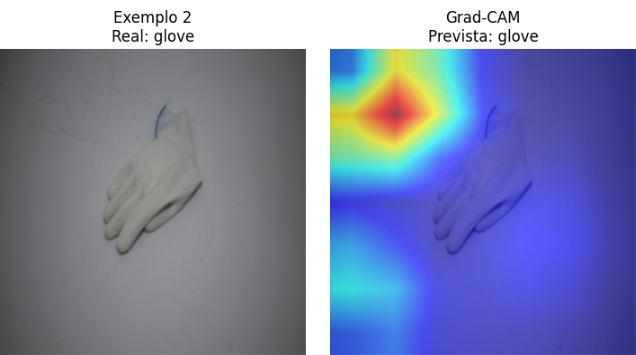
\includegraphics[width=0.74\textwidth]{gradcam_antes.png}
		\caption{Grad-CAM de uma luva antes da curadoria dos dados. A predição está correta, mas a ativação se concentra no fundo cinza, e não no objeto.}
		\label{fig:gradcam-antes}
	\end{figure}
	
	\subsection{Integração e limpeza: o que mudou}
	
	A reconstrução envolveu quatro frentes. Primeiro, a harmonização de rótulos da Tabela~\ref{tab:rotulos}, que reduziu o vocabulário a oito classes e removeu classes heterogêneas como \texttt{miscellaneous} e \texttt{trash}. Segundo, a curadoria semântica com CLIP, que separou 409 bitucas de cigarro do \texttt{plastic} do TrashBox e reuniu 1.317 embalagens longa vida na classe \texttt{tetra\_pack}. Terceiro, a deduplicação por MD5, dHash e pHash, que agrupou 35.603 imagens em 32.482 clusters e identificou 3.121 membros redundantes, mantidos no mesmo grupo para não vazarem entre os \emph{splits}. Quarto, a divisão por cluster, que impede que a mesma imagem apareça em lados diferentes da avaliação.
	
	O efeito sobre o Grad-CAM foi imediato. A Figura~\ref{fig:gradcam-depois} mostra duas predições corretas do modelo combinado: uma embalagem longa vida e uma pequena tampa plástica. Nos dois casos, o mapa cobre o objeto e não o fundo, o que é a evidência visual de que o modelo passou a usar a região relevante. A comparação com a Figura~\ref{fig:gradcam-antes} é o principal argumento deste trabalho de que a curadoria dos dados, e não apenas a troca de arquitetura, foi o que mudou o comportamento do modelo.
	
	\begin{figure}[htbp]
		\centering
		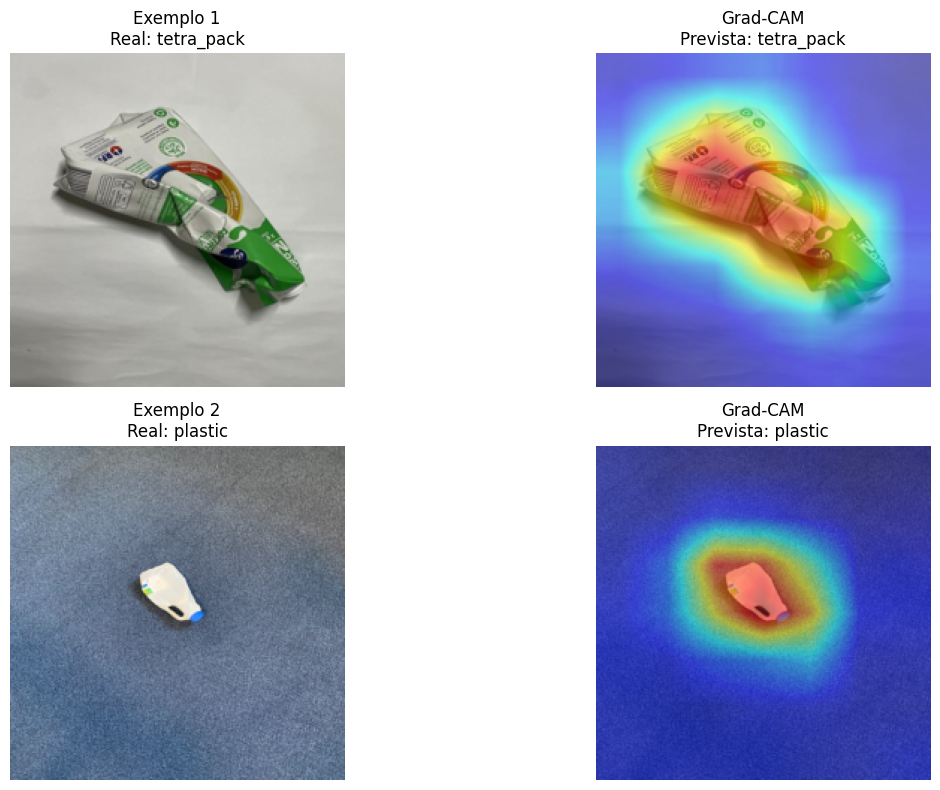
\includegraphics[width=0.60\textwidth]{gradcam_depois.png}
		\caption{Grad-CAM após a curadoria, no modelo combinado. A ativação acompanha o objeto (embalagem longa vida e tampa plástica) em vez de se dispersar pelo cenário.}
		\label{fig:gradcam-depois}
	\end{figure}
	
	\subsection{Desempenho no domínio de treino}
	
	A Tabela~\ref{tab:proprio} apresenta o desempenho de cada modelo no teste do próprio conjunto, na configuração de 50 épocas usada na avaliação cruzada. Os modelos treinados em uma única fonte vão bem no seu próprio domínio: 0,923 de acurácia no TrashBox, 0,907 no Kaggle e 0,998 no Roboflow. O valor do Roboflow é um alerta, e não um bom resultado: quase 100\% de acurácia em um conjunto com 1.392 imagens indica que a tarefa naquele domínio é fácil demais ou que restam atalhos, e a avaliação cruzada confirma a segunda hipótese.
	
	\begin{table}[htbp]
		\centering
		\small
		\caption{Desempenho no teste do próprio conjunto (modelos EfficientNet-B0, 50 épocas).}
		\label{tab:proprio}
		\begin{tabular}{lrrr}
			\toprule
			\textbf{Modelo treinado em} & \textbf{Acurácia} & \textbf{Macro-F1} & \textbf{Ac. balanceada} \\
			\midrule
			Kaggle & 0,907 & 0,898 & 0,902 \\
			TrashBox & 0,923 & 0,924 & 0,926 \\
			Roboflow & 0,998 & 0,998 & 0,998 \\
			Combinado & 0,896 & 0,904 & 0,924 \\
			\bottomrule
		\end{tabular}
	\end{table}
	
	O modelo combinado tem a menor acurácia no próprio teste (0,896), mas a acurácia balanceada (0,924) fica muito próxima dela. Isso é esperado: o teste combinado reúne as distribuições das quatro fontes, incluindo as classes mais difíceis, e é uma tarefa mais dura do que o teste de uma fonte isolada. A proximidade entre acurácia e acurácia balanceada mostra que o desempenho é distribuído de forma mais uniforme entre as classes, o que é o objetivo do treino por cotas por fonte. A Figura~\ref{fig:confusao} mostra a matriz de confusão correspondente: os erros se concentram entre \texttt{plastic} e \texttt{paper} (93 imagens de plástico classificadas como papel), entre \texttt{plastic} e \texttt{glass} (52) e entre \texttt{plastic} e \texttt{metal} (42), o que antecipa o padrão observado nas três arquiteturas.
	
	\begin{figure}[htbp]
		\centering
		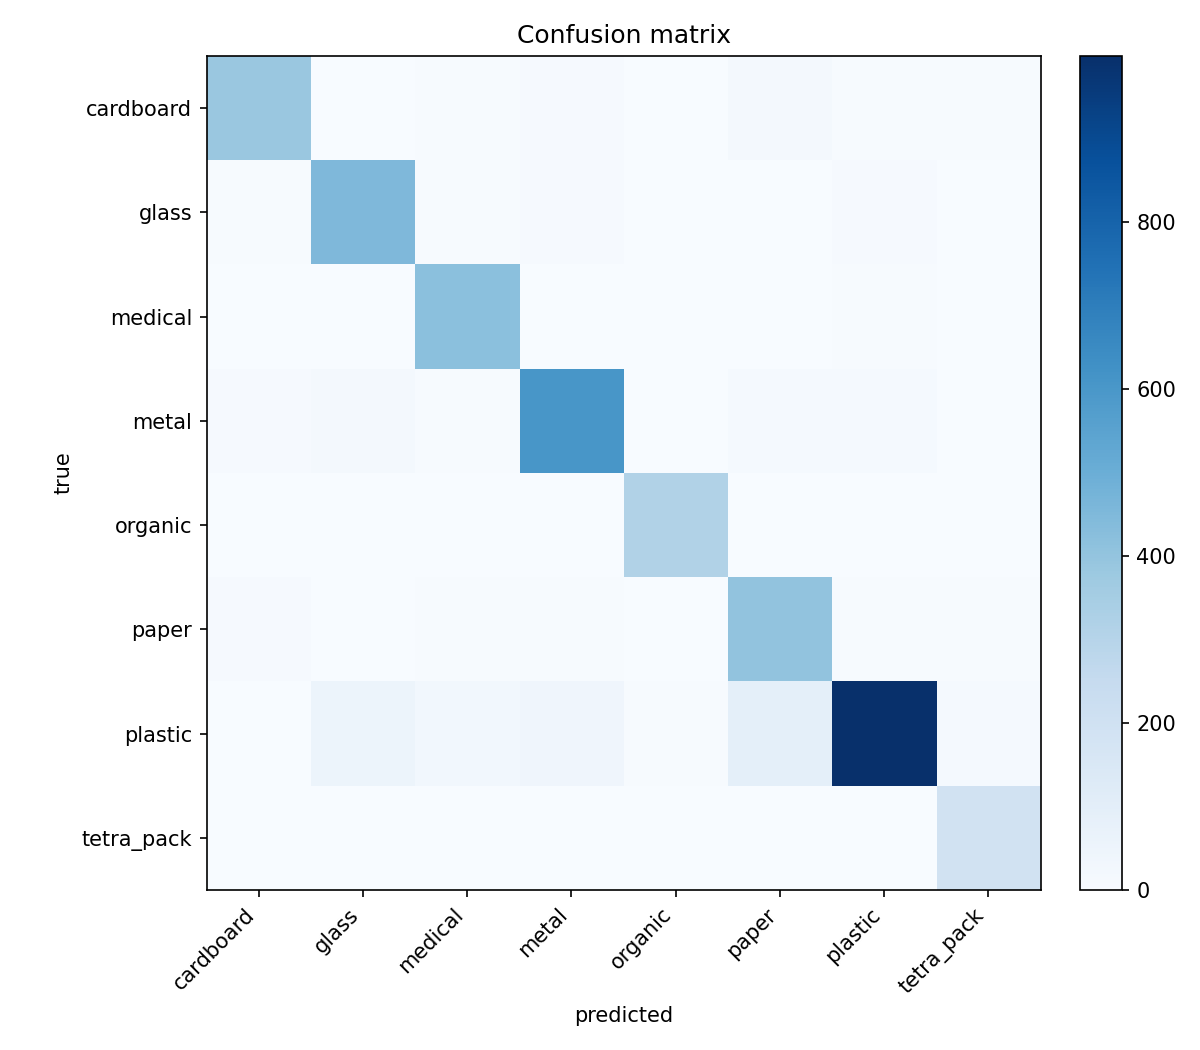
\includegraphics[width=0.55\textwidth]{matriz_confusao.png}
		\caption{Matriz de confusão do modelo combinado no teste (4.212 imagens, 50 épocas). A diagonal concentra os acertos; fora dela, a confusão se concentra entre \texttt{plastic} e \texttt{paper}, \texttt{plastic} e \texttt{glass}, e \texttt{plastic} e \texttt{metal}.}
		\label{fig:confusao}
	\end{figure}

	\subsection{Avaliação cruzada entre domínios}
	
	A Figura~\ref{fig:matriz-cruzada} apresenta a matriz completa de acurácia balanceada restrita. As células hachuradas são decomposições do próprio corpus (modelo ou alvo combinado) e ficam fora do \emph{ranking} entre domínios; a diagonal, em negrito, é a referência de desempenho no próprio conjunto.

	A Tabela~\ref{tab:cross} resume a comparação que importa, restrita às células verdadeiramente entre domínios e ao subconjunto comum de quatro classes. O modelo combinado lidera (0,798 de média), seguido pelo do Kaggle (0,771), do TrashBox (0,743) e do Roboflow (0,499). O \emph{gap} --- a diferença entre o desempenho no próprio domínio e a média fora dele --- conta a mesma história por outro ângulo: 0,113 para o combinado, 0,116 para o Kaggle, 0,196 para o TrashBox e 0,497 para o Roboflow. O modelo do Roboflow é o caso mais extremo: 0,997 no próprio conjunto e 0,499 fora dele.

	Duas ressalvas são necessárias. A primeira é que o modelo combinado tem apenas dois pares independentes (Garbage12 e RealWaste), porque as células internas foram excluídas; isso limita a comparação direta com os outros modelos, embora os dois conjuntos externos sejam a evidência mais limpa de mudança de domínio. A segunda é que a média completa da matriz, que inclui as decomposições internas, favorece artificialmente o modelo combinado (0,872 contra 0,751 do TrashBox, 0,733 do Kaggle e 0,506 do Roboflow), e por isso não é usada no \emph{ranking}.
	
	O pior par entre domínios foi o modelo do Roboflow aplicado ao teste do TrashBox: cobertura de 0,839, acurácia balanceada restrita de 0,339, Macro-F1 de 0,290 e acurácia de implantação de 0,113. A análise por classe mostra um padrão claro: 34,4\% dos \texttt{e-waste}, 47,5\% dos \texttt{plastic}, 30,4\% dos \texttt{metal} e 36,4\% dos \texttt{paper} foram classificados como \texttt{medical}. Para esse modelo, \texttt{medical} funciona como uma classe genérica para objetos que ele não reconhece fora do domínio de origem --- um sintoma de que a classe foi aprendida como ``o que não é as outras'' no conjunto de treino, e não como uma categoria visual.
	
	A cobertura precisa ser lida junto com a acurácia. No Garbage12, a cobertura é de apenas 0,295, porque \texttt{battery}, \texttt{clothes}, \texttt{shoes} e \texttt{trash} não existem no vocabulário dos modelos; por isso a acurácia de implantação fica entre 0,257 e 0,264, mesmo com a acurácia restrita perto de 0,90. No RealWaste, a cobertura é de 0,737, e a acurácia de implantação sobe para 0,44--0,47. Uma acurácia alta em um subconjunto pequeno de classes pode esconder a incapacidade de reconhecer classes ausentes, e é por isso que as duas métricas são reportadas juntas.
	
	\begin{figure}[htbp]
		\centering
		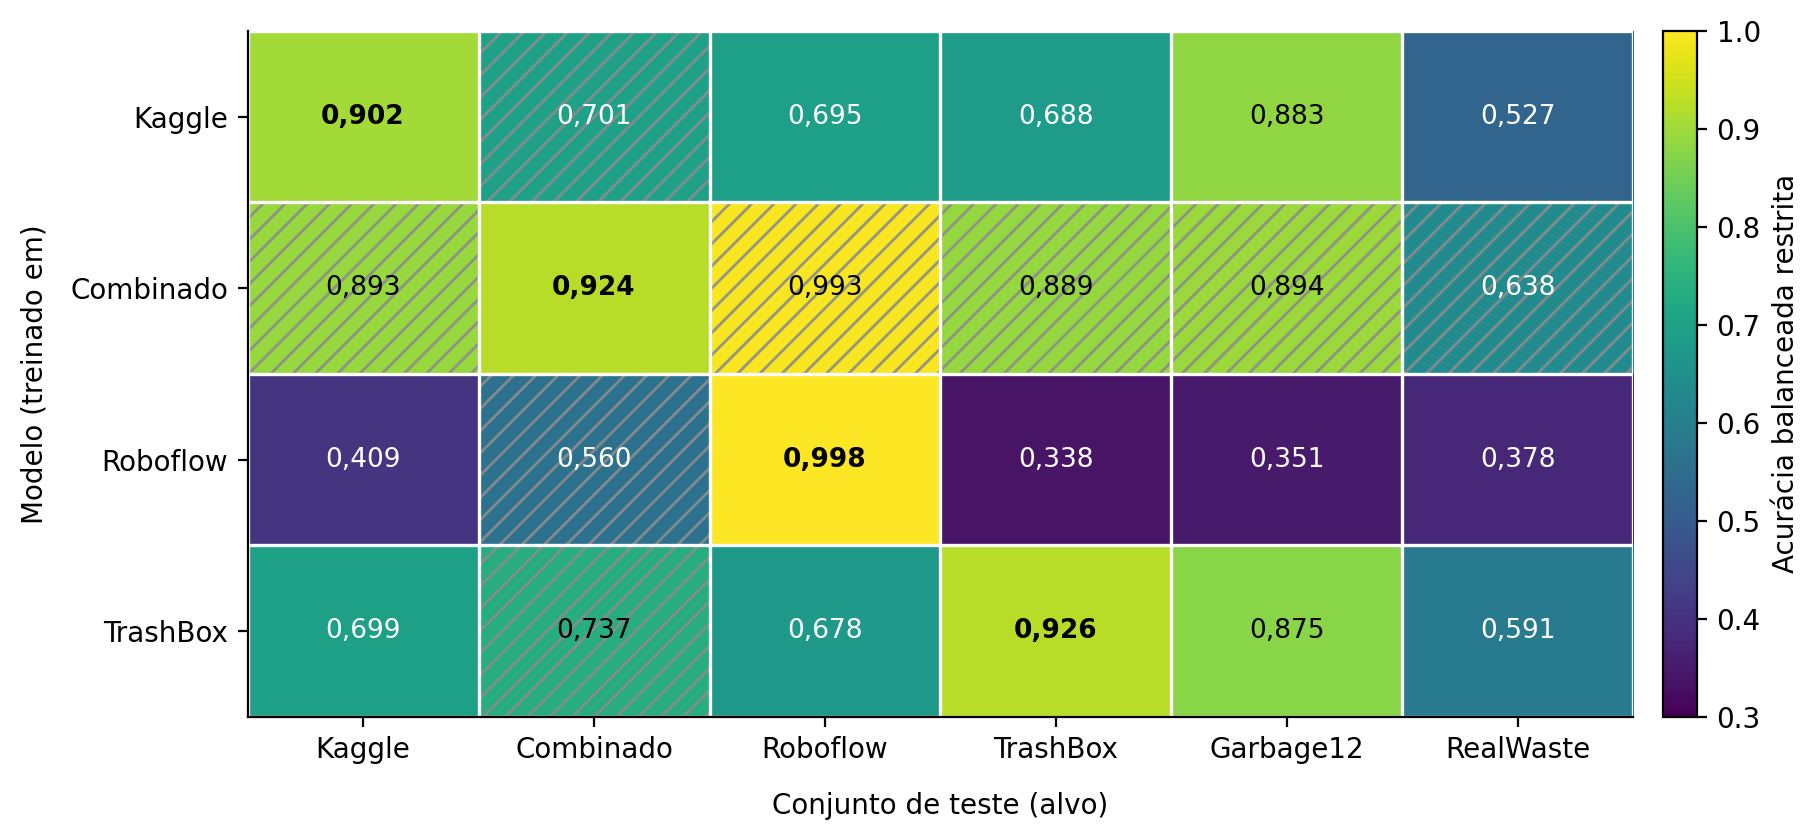
\includegraphics[width=0.96\textwidth]{matriz_cruzada.png}
		\caption{Acurácia balanceada restrita em todos os pares modelo $\times$ alvo. Células hachuradas são decomposições do corpus combinado (não são evidência independente de generalização); a diagonal em negrito é o desempenho no próprio conjunto.}
		\label{fig:matriz-cruzada}
	\end{figure}

	\begin{table}[htbp]
		\centering
		\small
		\caption{Comparação entre domínios no subconjunto comum de quatro classes.}
		\label{tab:cross}
		\begin{tabular}{lrrrrr}
			\toprule
			\textbf{Modelo} & \textbf{Pares} & \textbf{Próprio} & \textbf{Média entre domínios} & \textbf{\emph{Gap}} & \textbf{Cobertura} \\
			\midrule
			Combinado & 2 & 0,911 & \textbf{0,798} & 0,113 & 0,516 \\
			Kaggle & 4 & 0,887 & 0,771 & 0,116 & 0,568 \\
			TrashBox & 4 & 0,939 & 0,743 & 0,196 & 0,640 \\
			Roboflow & 4 & 0,997 & 0,499 & 0,497 & 0,647 \\
			\bottomrule
		\end{tabular}
	\end{table}

	\subsection{Otimização de hiperparâmetros}
	\label{sec:optuna}
	
	A Tabela~\ref{tab:optuna} compara o modelo com a configuração padrão ao modelo retreinado com a melhor configuração encontrada pelo Optuna. O modelo otimizado ficou ligeiramente abaixo do padrão em todas as métricas: $-0{,}0062$ de Macro-F1, $-0{,}0093$ de acurácia balanceada e $-0{,}0060$ de acurácia no teste do conjunto combinado.
	
	\begin{table}[htbp]
		\centering
		\small
		\caption{Configuração padrão versus configuração otimizada pelo Optuna, no conjunto combinado.}
		\label{tab:optuna}
		\begin{tabular}{lrrrrrr}
			\toprule
			\textbf{Modelo} & \textbf{Épocas} & \textbf{Melhor época} & \textbf{F1 val.} & \textbf{F1 teste} & \textbf{Ac. bal.} & \textbf{Acurácia} \\
			\midrule
			Padrão & 17 & 12 & 0,9257 & \textbf{0,9041} & \textbf{0,9237} & \textbf{0,8958} \\
			Otimizado & 24 & 19 & 0,9212 & 0,8979 & 0,9144 & 0,8898 \\
			\bottomrule
		\end{tabular}
	\end{table}
	
	A ausência de ganho tem explicações plausíveis. A busca avaliou cada tentativa com 12 épocas, enquanto o treinamento final teve até 50; a melhor configuração usa lotes menores (16) e imagens maiores (256), o que muda a dinâmica do treinamento em relação ao padrão (lote 256, imagem 224) e aumenta o custo por época. Com sete hiperparâmetros e 20 tentativas, a busca cobre apenas uma fração do espaço, e o ruído entre execuções pode ser da mesma ordem que a diferença observada. O resultado útil não é o ganho, e sim a constatação de que a configuração padrão já era competitiva: a otimização não é o gargalo do problema, e o esforço seguinte foi direcionado à comparação de arquiteturas e à avaliação externa.
	
	\subsection{Comparação de arquiteturas}
	
	As três arquiteturas foram retreinadas do zero com a mesma receita da Tabela~\ref{tab:hiper}, no mesmo conjunto combinado e com os mesmos \emph{splits}, de modo que a comparação isola a arquitetura. A Tabela~\ref{tab:arch} e a Figura~\ref{fig:curvas} mostram o resultado. O EfficientNet-B0 lidera em todas as métricas: 0,901 de Macro-F1 no teste, contra 0,894 do MobileNetV2 e 0,875 do ResNet18. O ResNet18, que é a rede mais pesada, é também a que menos acerta, e a diferença para o B0 (0,026) é maior do que a diferença entre B0 e MobileNetV2 (0,007). O valor do EfficientNet-B0 difere ligeiramente do registrado na Tabela~\ref{tab:proprio} (0,904 de Macro-F1) porque o modelo foi retreinado com a receita controlada de 30 épocas; a diferença de 0,003 é compatível com a variabilidade entre execuções e não altera a ordem.
	
	\begin{table}[htbp]
		\centering
		\small
		\caption{Desempenho das três arquiteturas no teste do conjunto combinado (4.212 imagens, 30 épocas de treino).}
		\label{tab:arch}
		\resizebox{\textwidth}{!}{%
			\begin{tabular}{lrrrrrrrr}
			\toprule
			\textbf{Modelo} & \textbf{Parâm.} & \textbf{GMACs} & \textbf{Épocas} & \textbf{Melhor} & \textbf{F1 val.} & \textbf{F1 teste} & \textbf{Ac. bal.} & \textbf{Acurácia} \\
			\midrule
			EfficientNet-B0 & 5,3 M & 0,39 & 17 & 12 & 0,925 & \textbf{0,901} & \textbf{0,921} & \textbf{0,893} \\
			MobileNetV2 & 3,5 M & 0,30 & 23 & 18 & 0,917 & 0,894 & 0,911 & 0,884 \\
			ResNet18 & 11,7 M & 1,81 & 28 & 23 & 0,907 & 0,875 & 0,897 & 0,867 \\
			\bottomrule
		\end{tabular}}
	\end{table}
	
	\begin{figure}[htbp]
		\centering
		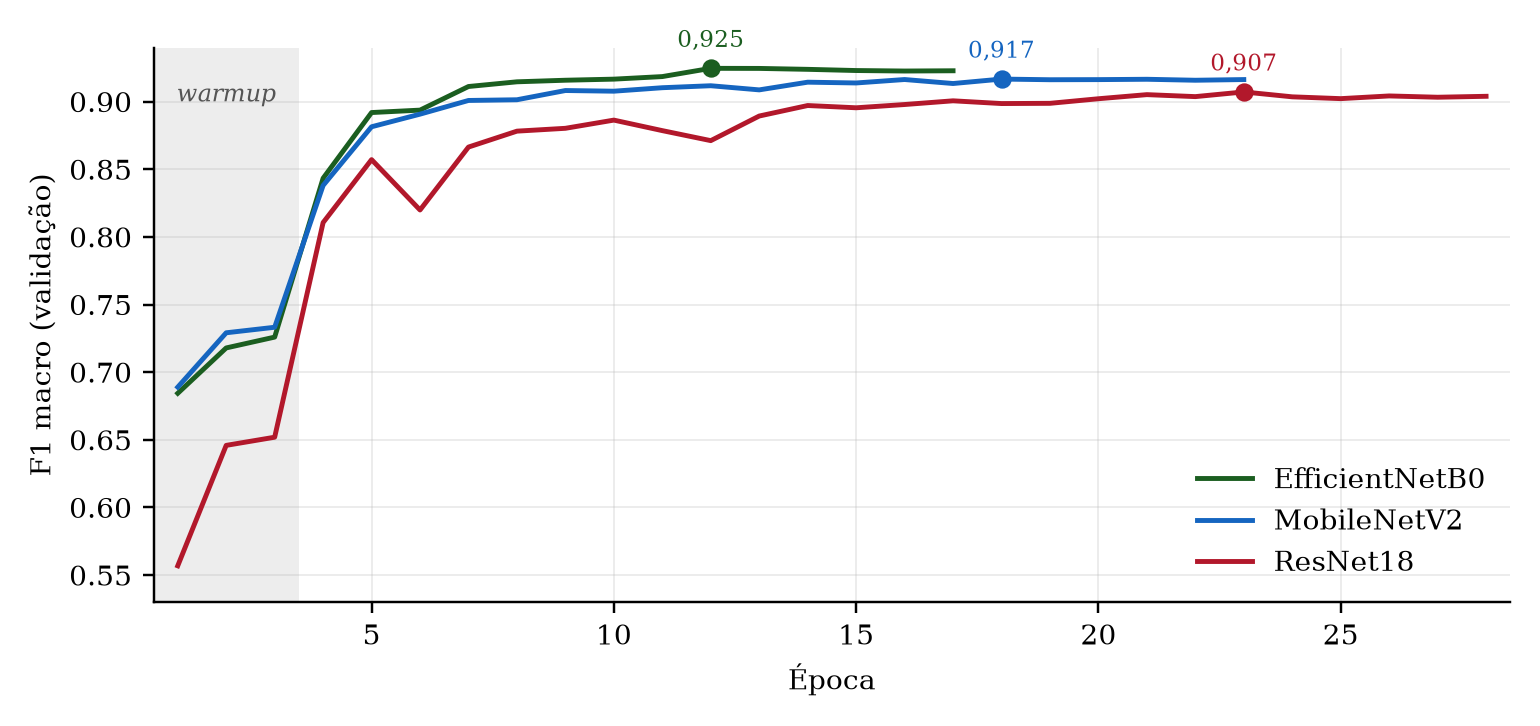
\includegraphics[width=0.94\textwidth]{curvas_f1.png}
		\caption{Macro-F1 de validação por época nas três arquiteturas. A faixa cinza marca as três épocas de \emph{warmup}; o marcador indica a melhor época de cada rede.}
		\label{fig:curvas}
	\end{figure}
	
	As curvas de validação têm o mesmo formato nas três redes: um salto entre a terceira e a quarta época, quando o \textit{backbone} é liberado, e depois ganho lento até o platô. Ao final do \emph{warmup}, o Macro-F1 era 0,725 no EfficientNet-B0, 0,733 no MobileNetV2 e 0,652 no ResNet18. Como o \emph{warmup} treina apenas a cabeça sobre um \textit{backbone} congelado, a diferença indica que as características do ResNet18 são menos separáveis por uma camada linear nesse conjunto antes do ajuste fino. Ele também demorou mais para chegar ao melhor ponto (época 23, contra 12 e 18).
	
	O custo ajuda a situar a diferença. O EfficientNet-B0 tem 5,3 milhões de parâmetros e 0,39 GMACs; o MobileNetV2 tem 3,5 milhões e 0,30 GMACs; o ResNet18 tem 11,7 milhões e 1,81 GMACs. O MobileNetV2 entrega 99,2\% do Macro-F1 do EfficientNet-B0 com cerca de dois terços dos parâmetros e três quartos das operações. O ResNet18 custa 4,6 vezes as operações do B0 e fica abaixo dos dois em desempenho. O tempo médio por época ficou entre 41 e 43 segundos nas três redes, o que sugere que o tempo foi dominado pelo carregamento das imagens e não pelo custo da rede; o número de épocas até o \emph{early stopping}, porém, acompanhou a dificuldade de ajuste.
	
	A Figura~\ref{fig:classe-f1} decompõe o F1 por classe. As maiores perdas estão nas mesmas classes nas três redes: \texttt{paper} tem o pior F1 (0,819, 0,803 e 0,787) e \texttt{plastic} tem o menor \emph{recall} (0,802, 0,808 e 0,783). A confusão é entre essas duas classes: 97 das 1.235 imagens de \texttt{plastic} do teste foram classificadas como \texttt{paper} pelo EfficientNet-B0, 92 pelo MobileNetV2 e 97 pelo ResNet18, o que derruba a precisão de \texttt{paper} (0,739 nas duas primeiras redes e 0,713 no ResNet18) apesar do \emph{recall} alto. O ResNet18 erra de forma um pouco diferente: 61 imagens de \texttt{plastic} foram para \texttt{medical}, contra 30 do B0 e 43 do MobileNetV2, e a precisão de \texttt{medical} cai de 0,888 para 0,843 e 0,789.
	
	\begin{figure}[htbp]
		\centering
		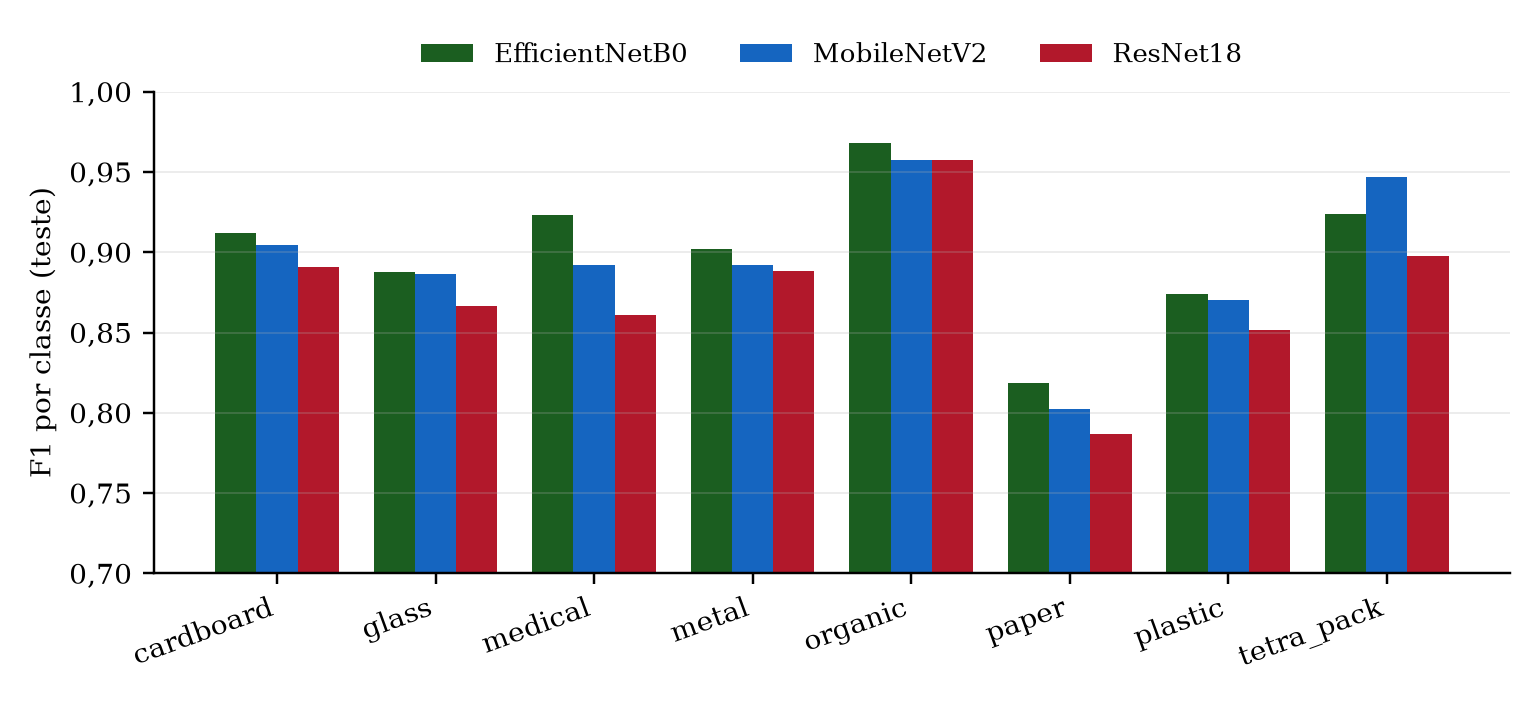
\includegraphics[width=0.94\textwidth]{f1_por_classe.png}
		\caption{F1 por classe no teste do conjunto combinado (4.212 imagens). \texttt{paper} e \texttt{plastic} concentram as maiores perdas nas três arquiteturas.}
		\label{fig:classe-f1}
	\end{figure}
	
	\subsection{Generalização externa das três arquiteturas}
	
	A comparação no domínio de treino poderia favorecer a rede mais expressiva. Para verificar se a ordem se mantém fora do domínio, os três \emph{checkpoints} foram avaliados no Garbage12 e no RealWaste, que não participaram de nenhum treinamento. A Tabela~\ref{tab:externa} e a Figura~\ref{fig:externa} mostram o resultado na interseção de seis classes; por usarem um subconjunto de classes diferente, esses valores não são diretamente comparáveis aos da Tabela~\ref{tab:cross}, que usa quatro classes.
	
	\begin{table}[htbp]
		\centering
		\small
		\caption{Acurácia balanceada restrita nas seis classes comuns, nos dois conjuntos externos.}
		\label{tab:externa}
		\begin{tabular}{lrrrr}
			\toprule
			\textbf{Modelo} & \textbf{Garbage12} & \textbf{RealWaste} & \textbf{Média} & \textbf{Implantação (média)} \\
			\midrule
			EfficientNet-B0 & 0,897 & \textbf{0,640} & \textbf{0,769} & \textbf{0,367} \\
			MobileNetV2 & \textbf{0,901} & 0,564 & 0,732 & 0,350 \\
			ResNet18 & 0,864 & 0,601 & 0,732 & 0,354 \\
			\bottomrule
		\end{tabular}
	\end{table}
	
	\begin{figure}[htbp]
		\centering
		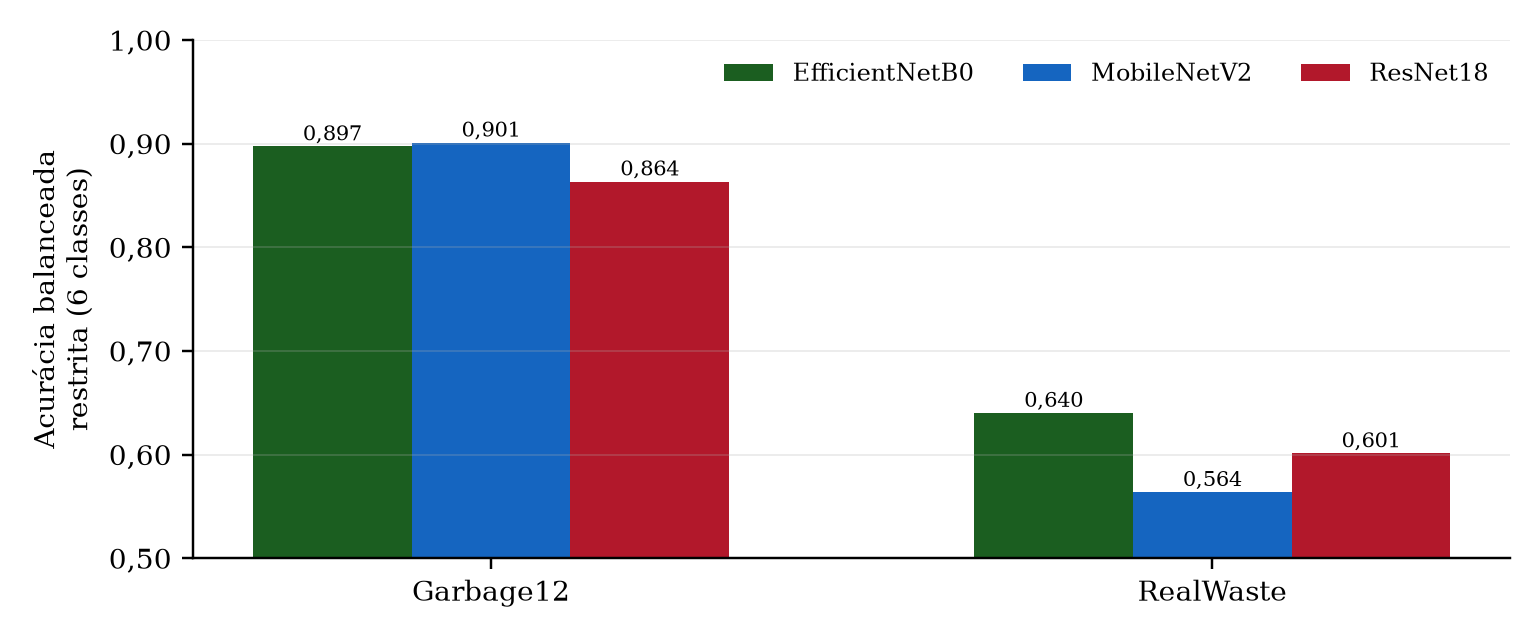
\includegraphics[width=0.84\textwidth]{avaliacao_externa.png}
		\caption{Acurácia balanceada restrita nas seis classes comuns, por conjunto externo.}
		\label{fig:externa}
	\end{figure}
	
	No Garbage12 as três redes ficam próximas, entre 0,864 e 0,901, e o MobileNetV2 é ligeiramente melhor que o EfficientNet-B0 (0,901 contra 0,897). A cobertura de 0,295 explica o restante: só 3.671 das 12.450 imagens pertencem a classes que os modelos conhecem. No RealWaste a ordem muda: o EfficientNet-B0 mantém a liderança (0,640), mas o ResNet18 passa o MobileNetV2 (0,601 contra 0,564). A diferença entre B0 e MobileNetV2 nesse conjunto (0,076) é dez vezes maior que a diferença entre os dois no teste combinado (0,007). A cobertura é 0,737, e a acurácia de implantação acompanha: 0,471, 0,439 e 0,451.
	
	No nível das classes, o padrão também não é o mesmo nos dois alvos. No Garbage12, \texttt{plastic} é a pior classe nas três redes (F1 entre 0,697 e 0,830), repetindo a dificuldade vista no teste combinado, e \texttt{glass} está entre as melhores (0,910 a 0,926). No RealWaste, \texttt{cardboard} e \texttt{glass} desabam (F1 entre 0,328 e 0,527), enquanto \texttt{organic} e \texttt{metal} se mantêm acima de 0,667. \texttt{glass} é a classe que mais depende do conjunto: vai de 0,910 no Garbage12 a 0,328 no RealWaste no caso do ResNet18.
	
	A leitura conjunta é que a vantagem do EfficientNet-B0 se mantém na média dos dois conjuntos externos (0,769, contra 0,732 do MobileNetV2 e 0,732 do ResNet18), mas não é uniforme. Com seis pares, diferenças de 0,001 entre MobileNetV2 e ResNet18 na média não devem ser lidas como separação real, e o que os dados sustentam é que as três redes têm dificuldade parecida quando o domínio muda. Nesse regime, o custo passa a ser o critério decisivo, e o MobileNetV2 se consolida como a alternativa leve ao EfficientNet-B0. O ResNet18, mesmo sendo a rede mais pesada, não trouxe ganho em nenhum dos dois regimes. As três \emph{runs} estão registradas no MLflow com seus artefatos, e a avaliação externa foi registrada como uma \emph{run} pai com seis \emph{runs} filhas, uma por par modelo $\times$ conjunto.
	
	\subsection{Explicabilidade e estudo de erros}
	
	O Grad-CAM final confirma a melhora, mas também expõe os limites do modelo. A Figura~\ref{fig:gradcam-falha} mostra um caso de falha: a imagem contém uma pequena tampa plástica sobre grama seca, a predição está correta, mas a ativação se concentra em uma região à esquerda, onde há outro fragmento claro, e não no objeto central. O padrão é o mesmo que aparecia antes da curadoria, em escala menor: o modelo ainda pode se apoiar em textura e em objetos vizinhos quando o alvo é pequeno em relação ao enquadramento.
	
	\begin{figure}[htbp]
		\centering
		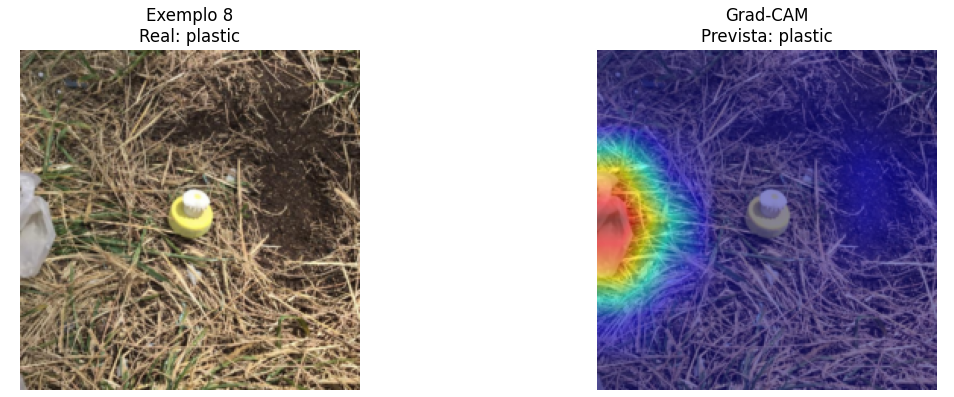
\includegraphics[width=0.78\textwidth]{gradcam_falha.png}
		\caption{Caso de falha residual: a classe está correta, mas a ativação se desloca para um fragmento vizinho, e não para o objeto central.}
		\label{fig:gradcam-falha}
	\end{figure}
	
	Essa limitação tem três causas prováveis. A primeira é a resolução do mapa: com $7 \times 7$ posições, o Grad-CAM destaca regiões, não contornos, e objetos pequenos ocupam poucas células. A segunda é a própria formulação de classificação de imagem inteira, que não separa o objeto do contexto e é sensível a múltiplos resíduos na cena. A terceira é a distribuição dos dados: mesmo após a curadoria, parte das imagens tem o objeto pequeno e o fundo dominante, e o modelo aprende a usar o contexto quando ele é preditivo. A mitigação natural é migrar para detecção ou segmentação, ou pelo menos recortar a região de interesse antes da classificação.
	
	\subsection{Implantação móvel}
	\label{sec:implantacao}
	
	O modelo final foi exportado para ONNX com três saídas em um único \emph{forward}: os \emph{logits} das oito classes, o mapa de ativação de $1280 \times 7 \times 7$ e a matriz de pesos $8 \times 1280$ da cabeça. As duas saídas extras permitem calcular o Grad-CAM no aparelho sem motor de gradientes e acrescentam poucos kilobytes ao grafo. O aplicativo Android, desenvolvido para o evento InovaTec, usa ONNX Runtime Mobile, não declara permissão de internet e executa a inferência localmente; o APK tem cerca de 62 MB, dos quais 16 MB são o modelo.
	
	A paridade entre PyTorch e ONNX foi verificada sobre as 4.212 imagens de teste, com concordância de top-1 igual a 1,000000, e os 24 \emph{fixtures} de teste do aplicativo passam com diferença máxima de probabilidade 0,0000. O Grad-CAM do aplicativo foi comparado ao mapa de referência do PyTorch e todas as células coincidem dentro de $2 \times 10^{-3}$. O limiar de confiança foi calibrado apenas na validação (nunca no teste): o valor 0,52 cobre 94\% das imagens com 95,1\% de acurácia entre as cobertas, e abaixo dele o aplicativo exibe um aviso de ``confiança baixa''. O aplicativo também foi projetado em torno do recorte: a guia de enquadramento é quadrada e a tela de resultado mostra a região avaliada, para que uma predição surpreendente possa ser rastreada até o que o modelo realmente viu.
	
	% ==========================================================
	\section{Conclusão e Trabalhos Futuros}
	\label{sec:conclusao}
	
	\textbf{Objetivos alcançados.} O trabalho partiu de dois problemas identificados na literatura --- a fragmentação dos conjuntos de dados e a opacidade dos modelos --- e mostrou que eles estão conectados. A integração das bases, com harmonização de rótulos assistida por CLIP e deduplicação por hashes exato e perceptual, produziu um conjunto de 15.707 imagens em oito classes, com isolamento verificado entre treino, validação e teste e \emph{pipeline} reprodutível em DVC. O protocolo de avaliação cruzada, com 24 pares modelo $\times$ alvo e seis pares adicionais nos conjuntos externos, mostrou que o modelo treinado no conjunto combinado generaliza melhor do que os modelos treinados em uma única fonte: 0,798 de acurácia balanceada média entre domínios, contra 0,771 do Kaggle, 0,743 do TrashBox e 0,499 do Roboflow, e 0,769 de média nos dois conjuntos externos contra 0,732 das outras duas arquiteturas. O Grad-CAM documentou o viés de fundo do primeiro modelo e a melhora após a curadoria, e o modelo foi implantado em um aplicativo Android com paridade exata e Grad-CAM no dispositivo.
	
	\textbf{Limitações.} A principal é a cobertura: os modelos têm oito classes e não sabem dizer ``não sei''. Nos conjuntos externos com classes ausentes, a acurácia de implantação cai para 0,26--0,47, mesmo com a acurácia restrita perto de 0,90. A segunda é a formulação de classe única por imagem, que não lida com múltiplos resíduos na cena nem com objetos pequenos. A terceira é a avaliação: os conjuntos externos têm tamanho moderado, os modelos foram treinados com uma única semente e não foram aplicados testes estatísticos pareados; diferenças de 0,001 não devem ser interpretadas como separação real. A quarta é a qualidade dos rótulos: a curadoria reduziu, mas não eliminou, erros herdados das bases, e a calibração do CLIP depende de inspeção manual. Por fim, o Grad-CAM é uma explicação de baixa resolução, de $7 \times 7$ posições, e não substitui uma análise de causalidade.
	
	\textbf{Trabalhos futuros.} Quatro direções parecem naturais. A primeira é substituir a classificação por detecção ou segmentação, o que resolve o problema de múltiplos objetos e de objetos pequenos e permite recortar a região de interesse antes de classificar. A segunda é aumentar a cobertura com um mecanismo de rejeição ou de classe ``desconhecida'', calibrado para manter a precisão entre as predições aceitas. A terceira é ampliar a avaliação: mais conjuntos externos, múltiplas sementes, intervalos de confiança por \emph{bootstrap} e testes pareados como o de McNemar \cite{dietterich1998}, além de seleção de modelo que nunca toque nos alvos externos \cite{gulrajani2021}. A quarta é a eficiência: quantização INT8 e avaliação de latência e consumo em dispositivos reais, com o MobileNetV2 como candidato natural para o modo leve.
	
	% ==========================================================
	\begin{thebibliography}{99}
		
		\bibitem{kaza2018}
		Silpa Kaza, Lisa Yao, Perinaz Bhada-Tata, and Frank Van Woerden.
		\textit{What a Waste 2.0: A Global Snapshot of Solid Waste Management to 2050}.
		World Bank, 2018.
		
		\bibitem{fotovvatikhah2025}
		F. Fotovvatikhah, I. Ahmedy, R. M. Noor, and M. U. Munir.
		A systematic review of AI-based techniques for automated waste classification.
		\textit{Sensors}, 25(10):3181, 2025.
		\url{https://doi.org/10.3390/s25103181}
		
		\bibitem{bawankule2023}
		R. Bawankule, V. Gaikwad, I. Kulkarni, S. Kulkarni, A. Jadhav, and N. Ranjan.
		Visual detection of waste using YOLOv8.
		In \textit{2023 International Conference on Sustainable Computing and Smart Systems (ICSCSS)}, pages 869--873, 2023.
		\url{https://doi.org/10.1109/ICSCSS57650.2023.10169688}
		
		\bibitem{shourie2024}
		P. Shourie, V. Anand, D. Upadhyay, S. Devliyal, and S. Gupta.
		Smart waste management: VGG16-based classification system for organic and recyclable materials.
		In \textit{2024 7th International Conference on Circuit Power and Computing Technologies (ICCPCT)}, volume 1, pages 1410--1414. IEEE, 2024.
		
		\bibitem{selvaraju2017}
		Ramprasaath R. Selvaraju, Michael Cogswell, Abhishek Das, Ramakrishna Vedantam, Devi Parikh, and Dhruv Batra.
		Grad-CAM: Visual explanations from deep networks via gradient-based localization.
		In \textit{Proceedings of the IEEE International Conference on Computer Vision (ICCV)}, pages 618--626, 2017.
		
		\bibitem{tan2019}
		Mingxing Tan and Quoc Le.
		EfficientNet: Rethinking model scaling for convolutional neural networks.
		In \textit{Proceedings of the 36th International Conference on Machine Learning (ICML)}, pages 6105--6114, 2019.
		
		\bibitem{sandler2018}
		Mark Sandler, Andrew Howard, Menglong Zhu, Andrey Zhmoginov, and Liang-Chieh Chen.
		MobileNetV2: Inverted residuals and linear bottlenecks.
		In \textit{Proceedings of the IEEE Conference on Computer Vision and Pattern Recognition (CVPR)}, pages 4510--4520, 2018.
		
		\bibitem{he2016}
		Kaiming He, Xiangyu Zhang, Shaoqing Ren, and Jian Sun.
		Deep residual learning for image recognition.
		In \textit{Proceedings of the IEEE Conference on Computer Vision and Pattern Recognition (CVPR)}, pages 770--778, 2016.
		
		\bibitem{akiba2019}
		Takuya Akiba, Shotaro Sano, Toshihiko Yanase, Takeru Ohta, and Masanori Koyama.
		Optuna: A next-generation hyperparameter optimization framework.
		In \textit{Proceedings of the 25th ACM SIGKDD International Conference on Knowledge Discovery \& Data Mining}, pages 2623--2631, 2019.
		
		\bibitem{radford2021}
		Alec Radford, Jong Wook Kim, Chris Hallacy, Aditya Ramesh, Gabriel Goh, Sandhini Agarwal, Girish Sastry, Amanda Askell, Pamela Mishkin, Jack Clark, Gretchen Krueger, and Ilya Sutskever.
		Learning transferable visual models from natural language supervision.
		In \textit{Proceedings of the 38th International Conference on Machine Learning (ICML)}, pages 8748--8763. PMLR, 2021.
		
		\bibitem{krawetz2013}
		Neal Krawetz.
		Kind of like that.
		\textit{The Hacker Factor Blog}, 21 January 2013.
		\url{https://www.hackerfactor.com/blog/index.php?/archives/529-Kind-of-Like-That.html}
		
		\bibitem{zauner2010}
		Christoph Zauner.
		\textit{Implementation and Benchmarking of Perceptual Image Hash Functions}.
		Master's thesis, Upper Austria University of Applied Sciences, Hagenberg Campus, 2010.
		\url{https://www.phash.org/docs/pubs/thesis_zauner.pdf}
		
		\bibitem{howardruder2018}
		Jeremy Howard and Sebastian Ruder.
		Universal language model fine-tuning for text classification.
		In \textit{Proceedings of the 56th Annual Meeting of the Association for Computational Linguistics}, pages 328--339, 2018.
		
		\bibitem{babe2025}
		A. Babé, R. Cuingnet, M. Scuturici, and S. Miguet.
		Generalization abilities of foundation models in waste classification.
		\textit{Waste Management}, 198:187--197, 2025.
		\url{https://doi.org/10.1016/j.wasman.2025.02.032}
		
		\bibitem{single2023}
		S. Single, S. Iranmanesh, and R. Raad.
		RealWaste: A novel real-life data set for landfill waste classification using deep learning.
		\textit{Information}, 14(12):633, 2023.
		\url{https://doi.org/10.3390/info14120633}
		
		\bibitem{kumsetty2022}
		N. Kumsetty, A. Bhat Nekkare, S. S., et al.
		TrashBox: Trash detection and classification using quantum transfer learning.
		In \textit{FRUCT 2022}, 2022.
		\url{https://doi.org/10.23919/FRUCT54823.2022.9770922}
		
		\bibitem{thung2016}
		G. Thung and M. Yang.
		Classification of trash for recyclability status.
		Technical report, Stanford University CS229, 2016.
		
		\bibitem{geirhos2020}
		Robert Geirhos, Jörn-Henrik Jacobsen, Claudio Michaelis, Richard Zemel, Wieland Brendel, Matthias Bethge, and Felix A. Wichmann.
		Shortcut learning in deep neural networks.
		\textit{Nature Machine Intelligence}, 2(11):665--673, 2020.
		
		\bibitem{azzahra2026}
		N. Azzahra, A. Hermawan, Junaedi, and K. Y. Edy.
		Impact of dataset background on deep learning-based waste classification.
		\textit{Jurnal RESTI}, 10(3):580--589, 2026.
		\url{https://doi.org/10.29207/resti.v10i3.6965}
		
		\bibitem{ijaz2026}
		M. Ijaz, S. U. R. Khan, A. U. Rehman, T. Asif, S. Vollmer, A. Dengel, and M. N. Asim.
		GlobalWasteData: A large-scale, integrated dataset for robust waste classification and environmental monitoring.
		arXiv:2602.07463, 2026.
		\url{https://arxiv.org/abs/2602.07463}
		
		\bibitem{dietterich1998}
		Thomas G. Dietterich.
		Approximate statistical tests for comparing supervised classification learning algorithms.
		\textit{Neural Computation}, 10(7):1895--1923, 1998.
		
		\bibitem{gulrajani2021}
		Ishaan Gulrajani and David Lopez-Paz.
		In search of lost domain generalization.
		In \textit{International Conference on Learning Representations (ICLR)}, 2021.
		
		\bibitem{kaggle_garbage}
		Arshnoor7389.
		Garbage classification dataset.
		Kaggle. \url{https://www.kaggle.com/datasets/arshnoor7389/garbage-classification-dataset}
		
		\bibitem{kaggle_garbage12}
		Mostafa Abla.
		Garbage classification (12 classes).
		Kaggle. \url{https://www.kaggle.com/datasets/mostafaabla/garbage-classification}
		
		\bibitem{roboflow_waste}
		Thesis Project SACR3.
		Classification model for waste materials in residential areas.
		Roboflow Universe. \url{https://universe.roboflow.com/thesis-project-sacr3/classification-model-for-waste-materials-in-residential-areas/dataset/4}
		
	\end{thebibliography}
	
\end{document}
